% =============================================================================
% MASTER THESIS: Time Series Approaches to Cocoa Price Risk
% Main LaTeX Document
% =============================================================================

\documentclass[12pt, a4paper]{article}

% -----------------------------------------------------------------------------
% PACKAGES
% -----------------------------------------------------------------------------

% Encoding and fonts
\usepackage[utf8]{inputenc}
\usepackage[T1]{fontenc}
\usepackage{lmodern}

% Language
\usepackage[english]{babel}

% Mathematics
\usepackage{amsmath}
\usepackage{amssymb}
\usepackage{mathtools}

% Graphics and figures
\usepackage{graphicx}
\usepackage{xcolor}
\definecolor{hohblue}{RGB}{0,45,114}  % University of Hohenheim blue
\graphicspath{{./figures/}{../images/}}  % Set paths for figures and logos
\usepackage{float}
\usepackage{caption}
\usepackage{subcaption}
\usepackage{threeparttable}  % For table notes

% Tables
\usepackage{booktabs}
\usepackage{tabularx}
\usepackage{longtable}
% \usepackage{multirow}  % not installed in MiKTeX

% Bibliography (biblatex with biber backend)
\usepackage[
    backend=biber,
    style=authoryear,
    sorting=nyt,
    maxcitenames=2,
    maxbibnames=99,
    uniquelist=false,
    url=false,
    doi=true,
    isbn=false
]{biblatex}
\addbibresource{references.bib}

% Cross-referencing
\usepackage{hyperref}
\hypersetup{
    colorlinks=true,
    linkcolor=blue,
    citecolor=blue,
    urlcolor=blue
}
\usepackage[capitalise, noabbrev]{cleveref}

% Page layout
\usepackage[
    top=2.5cm,
    bottom=2.5cm,
    left=3cm,
    right=2.5cm
]{geometry}

% Line spacing
\usepackage{setspace}
\onehalfspacing

% Headers and footers
\usepackage{fancyhdr}
\pagestyle{fancy}
\fancyhf{}
\fancyhead[L]{\leftmark}
\fancyhead[R]{\thepage}
\renewcommand{\headrulewidth}{0.4pt}

% Code listings (if needed)
\usepackage{listings}
\lstset{
    basicstyle=\ttfamily\small,
    breaklines=true,
    frame=single
}

% Appendix
\usepackage[toc,page]{appendix}

% -----------------------------------------------------------------------------
% CUSTOM COMMANDS
% -----------------------------------------------------------------------------

% Commonly used symbols
\newcommand{\E}{\mathbb{E}}           % Expectation
\newcommand{\Var}{\text{Var}}         % Variance
\newcommand{\Cov}{\text{Cov}}         % Covariance
\newcommand{\VaR}{\text{VaR}}         % Value at Risk
\newcommand{\RV}{\text{RV}}           % Realized Volatility
\newcommand{\HAR}{\text{HAR}}         % HAR model
\newcommand{\ENSO}{\text{ENSO}}       % ENSO index

% Operators
\DeclareMathOperator*{\argmin}{arg\,min}
\DeclareMathOperator*{\argmax}{arg\,max}

% Quantile notation
\newcommand{\Qtau}{Q_{\tau}}          % Conditional quantile

% -----------------------------------------------------------------------------
% DOCUMENT INFO
% -----------------------------------------------------------------------------

\title{Time Series Approaches to Cocoa Price Risk}
\author{Felix Köhler}
\date{\today}

% =============================================================================
% DOCUMENT
% =============================================================================

\begin{document}

% -----------------------------------------------------------------------------
% FRONT MATTER
% -----------------------------------------------------------------------------

\pagenumbering{roman}

% Title page
\begin{NoHyper}
\begin{titlepage}
    \centering
    \vspace*{0.5cm}

    % --- Title (very top) ---
    {\LARGE\bfseries Time Series Approaches to Cocoa Price Risk\par}

    \vspace{1.8cm}

    % --- Logos: University (left) and Ritter Sport (right) ---
    \begin{minipage}[c]{0.5\textwidth}
        \centering
        \includegraphics[width=0.85\textwidth]{Uni_Logo_quadr.png}
    \end{minipage}\hfill
    \begin{minipage}[c]{0.5\textwidth}
        \centering
        \includegraphics[width=0.62\textwidth]{RS_Logo.png}
    \end{minipage}

    \vspace{2cm}

    % --- Author ---
    {\large\bfseries Felix Köhler\par}
    \vspace{0.3cm}
    {\normalsize Matriculation Number: 839611\par}

    \vspace{1cm}

    {\normalsize Department of Business Mathematics and Data Science (510G)\par}

    \vspace{1cm}

    {\normalsize
        Master Thesis submitted in partial fulfilment of the requirements for the\\
        degree of Master of Science in Agricultural Sciences --\\
        Advisory and Innovation Services in Agri-Food Systems\par}

    \vspace{1cm}

    {\normalsize June 2026\par}

    \vspace{1cm}

    {\normalsize Supervisor: Prof.\ Dr.\ Thomas Dimpfl \\ Second Supervisor: Dr.\ Johannes Bleher\par}

    \vfill
\end{titlepage}
\end{NoHyper}

% Abstract (placeholder)
% \section*{Abstract}
% \addcontentsline{toc}{section}{Abstract}

% [Abstract will be written after empirical results are complete.]

% Table of contents
\newpage
\pagestyle{empty}
\tableofcontents

% List of figures (optional)
% \listoffigures
% \addcontentsline{toc}{section}{List of Figures}

% List of tables (optional)
% \listoftables
% \addcontentsline{toc}{section}{List of Tables}

% -----------------------------------------------------------------------------
% MAIN MATTER
% -----------------------------------------------------------------------------

\newpage
\pagestyle{fancy}
\pagenumbering{arabic}

% Section 0: Abstract
\section*{Abstract}
\addcontentsline{toc}{section}{Abstract}

This thesis asks two questions: whether Heterogeneous Autoregressive (HAR) quantile regression produces better out-of-sample distributional forecasts of cocoa futures volatility than established benchmarks, and whether augmenting the model with the El~Ni\~no--Southern Oscillation (ENSO) climate index improves long-horizon upper-tail forecasts. Daily Open-High-Low-Close prices for ICE London cocoa front-month futures spanning January~1985 to December~2025 (10,376 trading days) are used to construct a Yang-Zhang volatility proxy, validated against realized volatility from approximately one year of five-minute intraday data. Forecasts at six horizons (1~day to 12~months) are evaluated by quantile loss and QLIKE against five competing models, with Model Confidence Sets used to assess statistical significance.

On the first question, the value of direct quantile estimation is concentrated at short horizons. HAR-QR delivers the lowest upper-tail ($\tau = 0.95$) quantile loss from one day through three months, and at one day and one week it is the sole top-ranked model in a 90\% Model Confidence Set that excludes historical volatility, GARCH(1,1), and the HAR-OLS pseudo-quantile. The ranking then reverses: the HAR-OLS pseudo-quantile overtakes HAR-QR at six months, and GARCH(1,1) is the best upper-tail forecaster at twelve months, 29\% below HAR-QR in quantile loss, though these long-horizon differences are not statistically significant. For mean forecasts, HAR-OLS dominates at every horizon under QLIKE, MSE, and MAE. Upper-quantile coverage is near the nominal $5\%$ at one day and one week but deteriorates as the horizon lengthens, reaching 14.6\% at twelve months.

On the second question, the Ni\~no~3.4 index worsens upper-tail quantile loss at every horizon from one to six months and improves it by only $3.3\%$ at twelve months. Three robustness diagnostics dissolve even this residual gain: it is confined entirely to the 2022--2024 cocoa supply-crisis window---in the pre-crisis subsample ENSO augmentation \emph{raises} twelve-month upper-tail loss by 16\%---it follows a lag structure that contradicts the agronomic transmission hypothesis, and it does not replicate on Arabica coffee or raw sugar. ENSO therefore yields no robust forecast improvement at any horizon; its apparent long-horizon value is a regime-conditional, sample-specific artefact rather than a replicable structural climate channel.

The thesis makes three contributions: the first application of HAR-QR to an agricultural commodity, the first evaluation at horizons extending to twelve months, and the first empirical test of an ENSO-augmented HAR-QR specification for cocoa.

\vspace{0.5cm}
\noindent\textbf{Keywords:} cocoa futures, volatility forecasting, HAR model, quantile regression, ENSO, long-horizon forecasting, Yang-Zhang estimator

\newpage
% Section 1: Introduction
\input{01_Introduction}
\newpage
% Section 2: Literature Review
\input{02_LiteratureReview}
\newpage
% Section 3: Methodology
\section{Methodology}
\label{sec:methodology}

This section specifies the econometric framework for forecasting cocoa futures
volatility at horizons from one day to twelve months. We first define the
volatility measure, then specify the HAR-QR model and its ENSO-augmented
extension, describe the benchmark models, and finally lay out the evaluation
framework. Table~\ref{tab:model-overview} provides an at-a-glance summary of
the five models before the detailed specifications follow.

\begin{table}[htbp]
\small
\caption{Overview of models compared in this study, ordered from simplest to
most complex.}
\label{tab:model-overview}
\noindent\hspace*{-1.25cm}\begin{tabular}{lccccc}
\toprule
 & \multicolumn{3}{c}{Benchmarks} & \multicolumn{2}{c}{Main models} \\
\cmidrule(lr){2-4}\cmidrule(lr){5-6}
Feature & Hist.\ Vol. & GARCH(1,1) & HAR-OLS & HAR-QR & HAR-X-QR \\
\midrule
Model class         & Non-param.     & ARCH-type    & Linear reg.    & Quantile reg.  & Quantile reg.  \\
HAR lags ($d/w/m$)  & No             & No           & Yes            & Yes            & Yes            \\
ENSO regressor      & No             & No           & No             & No             & Yes            \\
Quantile output     & Empirical      & Simulation   & None           & Direct         & Direct         \\
Estimation          & ---            & MLE          & OLS            & Check fn.      & Check fn.      \\
Multi-period design & Rolling window & Recursive    & Direct         & Direct         & Direct         \\
Thesis role         & Naive BM       & Param.\ BM   & HAR benchmark  & Main (RQ1)     & Main (RQ2)     \\
\bottomrule
\end{tabular}
\par\smallskip
{\footnotesize Direct = horizon-specific model estimated by direct projection;
Recursive = closed-form GARCH mean recursion, quantiles via Gaussian closed-form
(Eq.~\ref{eq:garch-quantile}); Check fn.\ = check-function (quantile) loss;
BM = benchmark; Hist.\ Vol.\ = rolling 252-day window with empirical quantiles.}
\end{table}

%------------------------------------------------------------------------------
\subsection{Volatility Measure}
\label{sec:meth-vol-measure}
%------------------------------------------------------------------------------

We measure daily volatility using the Yang-Zhang estimator, which combines
overnight and trading-session variance components:
\begin{equation}
\label{eq:yang-zhang}
\hat{\sigma}^2_{\text{YZ}} = \hat{\sigma}^2_O + k \hat{\sigma}^2_C + (1-k) \hat{\sigma}^2_{\text{RS}},
\end{equation}
where $\hat{\sigma}^2_O$ captures overnight variance, $\hat{\sigma}^2_C$
captures open-to-close variance, and $\hat{\sigma}^2_{\text{RS}}$ is the
Rogers-Satchell component that exploits the daily range. The weighting
factor $k = 0.34/(1.34 + (n+1)/(n-1))$ minimizes estimator variance.

This choice is motivated by two considerations. First, Yang-Zhang achieves
efficiency gains over close-to-close estimators and second,
it can be computed over our full 40-year daily sample, unlike realized volatility
which requires high-frequency data. We validate
the Yang-Zhang proxy against five-minute realized volatility in
Section~\ref{sec:data}, comparing rolling-window aggregates (22-day
averages) of both measures via a Mincer-Zarnowitz regression. This
comparison at the multi-day level aligns with the HAR model's use of
averaged volatility as both predictors and targets.

%------------------------------------------------------------------------------
\subsection{The HAR-QR Model}
\label{sec:meth-har-qr}
%------------------------------------------------------------------------------

Combining the HAR framework with quantile regression yields the HAR-QR
model. The HAR-QR model for horizon $h$ and quantile $\tau$ is
\begin{equation}
\label{eq:har-qr}
Q_{\tau}(\bar{\sigma}_{t:t+h} \mid \mathcal{F}_t) = \beta_0(\tau) + \beta_d(\tau) \sigma_t^{(d)} + \beta_w(\tau) \sigma_t^{(w)} + \beta_m(\tau) \sigma_t^{(m)},
\end{equation}
where $\mathcal{F}_t$ denotes the information set at time $t$. The
volatility components capture variation at three frequencies:
\begin{align}
\sigma_t^{(d)} &= \sigma_t, \label{eq:har-daily} \\
\sigma_t^{(w)} &= \frac{1}{5} \sum_{i=0}^{4} \sigma_{t-i}, \label{eq:har-weekly} \\
\sigma_t^{(m)} &= \frac{1}{22} \sum_{i=0}^{21} \sigma_{t-i}. \label{eq:har-monthly}
\end{align}

The key feature of quantile regression is that each quantile $\tau$ has its
own coefficient vector, allowing the relationship between predictors and
future volatility to differ across the distribution. For the median
($\tau = 0.50$), the coefficients may resemble those from OLS estimation.
For the upper quantile ($\tau = 0.95$), the coefficients capture how the
predictors relate to volatility during high-volatility episodes. We report three quantiles: $\tau \in \{0.50, 0.75, 0.95\}$. The median
$\tau = 0.50$ serves as an anchor to OLS-based point forecasts. The
intermediate quantile $\tau = 0.75$ traces the transition from central
to tail behaviour. The upper quantile $\tau = 0.95$ is of primary
interest, as it captures the conditional upper bound of volatility, the
regime where mean forecasts are most likely to understate actual outcomes.
Lower quantiles ($\tau = 0.05$, $0.25$) are omitted as the thesis focuses
on upper-tail risk.

The dependent variable is the average daily volatility over the forecast
horizon, following the HAR literature convention
\parencite{ghyselsDirectIteratedMultiperiod2019,
clementsHarvestingHARXVolatility2024}:
\begin{equation}
\label{eq:horizon-vol}
\bar{\sigma}_{t:t+h} = \frac{1}{h} \sum_{i=1}^{h} \sigma_{t+i}.
\end{equation}
This averaging ensures comparability across horizons and aligns with the
HAR model's construction, where weekly and monthly components are themselves
averages of daily volatility.

We adopt the \emph{direct} forecasting approach: a separate model is
estimated for each horizon $h$, using $\bar{\sigma}_{t:t+h}$ as the
dependent variable. This contrasts with \emph{iterated} forecasting, which
estimates a one-step model and iterates forward.
\textcite{ghyselsDirectIteratedMultiperiod2019} find that direct forecasting
is preferred for realized volatility models. For quantile regression,
direct estimation is particularly natural, as it produces the conditional
quantile at horizon $h$ without the distributional assumptions required to
iterate quantile forecasts. Our longest horizons (6--12 months) would
require iterating hundreds of daily steps, amplifying any model
misspecification.

We estimate HAR-QR at six horizons: $h \in \{1, 5, 22, 66, 132, 264\}$
trading days, corresponding to 1~day, 1~week, 1~month, 3~months, 6~months,
and 12~months. The short horizons (1~day to 1~month) serve to validate the
methodology against existing literature: HAR-QR has been tested at horizons
up to 22 trading days \parencite{lyocsaImprovingStockMarket2021}. The long
horizons (6 and 12 months) constitute the core contribution, testing
whether HAR-QR can produce useful forecasts at horizons where no prior study
has ventured.

At long horizons, the autoregressive signal from lagged volatility fades.
We therefore augment the HAR-QR model with the ENSO climate index:
\begin{equation}
\label{eq:har-x-qr}
Q_{\tau}(\bar{\sigma}_{t:t+h} \mid \mathcal{F}_t) = \beta_0(\tau) + \beta_d(\tau) \sigma_t^{(d)} + \beta_w(\tau) \sigma_t^{(w)} + \beta_m(\tau) \sigma_t^{(m)} + \gamma(\tau) \text{ENSO}_t,
\end{equation}
We refer to this augmented specification as the \emph{HAR-X-QR} model,
where the ``-X'' suffix denotes the inclusion of the exogenous ENSO regressor.
Here $\text{ENSO}_t$ is the Ni\~no~3.4 sea surface temperature anomaly
index from NOAA, measured monthly. The coefficient $\gamma(\tau)$ captures
the marginal effect of ENSO conditions on future volatility at quantile
$\tau$.

We use \emph{contemporary} ENSO, meaning $\text{ENSO}_t$ predicts
$\bar{\sigma}_{t:t+h}$, rather than explicitly lagged ENSO values. This
specification is standard in the climate-commodity literature
\parencite{bouriNinoForecastabilityOilprice2021,
bonatoNinoNinaForecastability2023} and is causal: the Ni\~no~3.4
anomaly for month $t$ is publicly observable before any forecast is issued,
so no forward-looking information enters the model. The sensitivity of this
specification to alternative ENSO lags is examined in
Section~\ref{sec:res-robustness}.

Positive Ni\~no~3.4 anomalies indicate El~Ni\~no conditions; negative
anomalies indicate La~Ni\~na. Full details of the index construction,
sample coverage, and monthly-to-daily alignment are provided in
Section~\ref{sec:data-enso}.

The HAR-QR model is estimated by minimizing the check function loss:
\begin{equation}
\label{eq:har-qr-estimation}
\hat{\beta}(\tau) = \argmin_{\beta} \sum_{t=1}^{T-h} \rho_{\tau}(\bar{\sigma}_{t:t+h} - X_t' \beta),
\end{equation}
where $X_t = (1, \sigma_t^{(d)}, \sigma_t^{(w)}, \sigma_t^{(m)})'$ for the
basic model, or
$X_t = (1, \sigma_t^{(d)}, \sigma_t^{(w)}, \sigma_t^{(m)}, \text{ENSO}_t)'$
for the extended model. The check function is defined as:
\begin{equation}
\label{eq:check-function}
\rho_{\tau}(u) = u \cdot (\tau - \mathbf{1}_{u < 0}) =
\begin{cases}
\tau \cdot u & \text{if } u \geq 0, \\
(\tau - 1) \cdot u & \text{if } u < 0.
\end{cases}
\end{equation}
This asymmetric loss function penalizes under-prediction more heavily when
$\tau$ is large and over-prediction more heavily when $\tau$ is small,
ensuring that the estimated quantile achieves the target coverage rate. The
minimization is a linear programming problem solved efficiently using the
simplex algorithm \parencite{koenker1987algorithm}. Standard errors are
computed using the bootstrap.

%------------------------------------------------------------------------------
\subsection{Benchmark Models}
\label{sec:meth-benchmarks}
%------------------------------------------------------------------------------

We compare HAR-QR and HAR-X-QR against three benchmarks that span the major modeling
paradigms discussed in the literature review.

The first benchmark is \emph{rolling historical volatility} with a one-year
window ($w = 252$):
\begin{equation}
\label{eq:hist-vol}
\hat{\sigma}_{t+h}^{\text{hist}} = \sqrt{\frac{1}{w} \sum_{i=1}^{w} (r_{t-i+1} - \bar{r})^2}.
\end{equation}
For quantile forecasts, we compute empirical quantiles of the historical
volatility distribution: sort the $w$ past volatilities and select the
value at position $\lceil \tau \cdot w \rceil$. This model captures only
unconditional variation and serves as a naive baseline.

The second benchmark is the \emph{GARCH(1,1)} model
\parencite{bollerslev1986generalized}:
\begin{equation}
\label{eq:garch}
\sigma_t^2 = \omega + \alpha \varepsilon_{t-1}^2 + \beta \sigma_{t-1}^2.
\end{equation}
For mean forecasts at horizon $h$, the GARCH(1,1) produces closed-form
predictions:
\begin{equation}
\label{eq:garch-forecast}
\E_t[\sigma_{t+h}^2] = \bar{\sigma}^2 + (\alpha + \beta)^{h-1}(\sigma_{t+1}^2 - \bar{\sigma}^2),
\end{equation}
where $\bar{\sigma}^2 = \omega / (1 - \alpha - \beta)$ is the unconditional
variance and $(\alpha + \beta)^{h-1}$ governs the speed of mean reversion.
At long horizons, all $h$-step forecasts converge to $\bar{\sigma}^2$,
irrespective of current conditions, a structural limitation of daily
GARCH at 6--12 month horizons.

For quantile forecasts we adopt a closed-form Gaussian approach consistent
with the normal-innovation assumption used in estimation.
The mean forecast $\hat{\sigma}_{t,h}$ is obtained as the square root of
the average $h$-step variance, $\hat{\sigma}_{t,h} = \sqrt{h^{-1}\sum_{k=1}^{h}\E_t[\sigma_{t+k}^2]}$.
Forecast uncertainty is captured by the in-sample standard deviation
$s_t$ of daily volatility over the estimation window. The $\tau$-quantile
forecast is then
\begin{equation}
\label{eq:garch-quantile}
\hat{Q}_{\tau,t}^{\text{GARCH}} = \hat{\sigma}_{t,h} + \Phi^{-1}(\tau)\, s_t,
\end{equation}
where $\Phi^{-1}(\tau)$ is the standard normal quantile function.

The third benchmark is \emph{HAR-OLS}, the standard HAR model estimated
by ordinary least squares. OLS yields only a conditional mean forecast
$\hat{\mu}_{t,h}$, but a distributional forecast can be constructed from
the in-sample residuals. Let $\hat{\varepsilon}_i = \sigma_i - \hat{\mu}_i$
denote the residuals from the training window. The $\tau$-quantile forecast
is then
\begin{equation}
\label{eq:har-ols-quantile}
\hat{Q}_{\tau,t}^{\text{OLS}} = \hat{\mu}_{t,h} + \hat{F}^{-1}_{\varepsilon}(\tau),
\end{equation}
where $\hat{F}^{-1}_{\varepsilon}(\tau)$ is the empirical $\tau$-quantile of
the training-window residuals. This pseudo-quantile approach requires no
distributional assumption and produces forecasts that are directly comparable
to HAR-QR: if HAR-QR provides no improvement over HAR-OLS at quantile $\tau$,
then conditioning on the HAR structure suffices and quantile regression adds
no value. Comparing the two at $\tau = 0.50$ tests symmetry of the conditional
distribution; comparing at $\tau = 0.95$ tests whether the upper tail is
better captured by explicit quantile estimation.

%------------------------------------------------------------------------------
\subsection{Evaluation Framework}
\label{sec:meth-evaluation}
%------------------------------------------------------------------------------

Evaluating volatility forecasts is complicated by the fact that volatility
is unobserved, and every evaluation compares forecasts against an imperfect
proxy \parencite{pattonVolatilityForecastComparison}. We evaluate forecasts
against Yang-Zhang volatility computed from realized prices, using loss
functions that \textcite{pattonVolatilityForecastComparison} has shown to
be robust to noise in the volatility proxy.

For mean and median forecasts, we use QLIKE as the primary metric. All five models are therefore compared on QLIKE: the three benchmarks contribute their mean forecasts, while HAR-QR and HAR-X-QR contribute their median ($\tau = 0.50$) forecasts, which provide a natural reference point for comparison with OLS-based point forecasts.
\begin{equation}
\label{eq:qlike}
\text{QLIKE} = \frac{1}{T} \sum_{t=1}^{T} \left( \log \hat{\sigma}_t^2 + \frac{\sigma_t^2}{\hat{\sigma}_t^2} \right).
\end{equation}
\textcite{pattonVolatilityForecastComparison} derives necessary and
sufficient conditions for the loss function to yield forecast rankings that
are robust to proxy noise, showing that among nine commonly used loss
functions, only MSE and QLIKE satisfy these conditions. We prefer QLIKE
because it penalizes under-prediction of volatility proportionally more than
MSE, which is appropriate when under-prediction is costlier than
over-prediction, a property particularly relevant for upper-quantile
forecasts. As \textcite{pukeCoherentForecastingRealized2026} demonstrate,
aligning estimation and evaluation loss functions, what they call
\emph{coherent forecasting}, yields significant accuracy gains. Our HAR-QR
models are coherent by construction: the check function
(Equation~\ref{eq:check-function}) serves as both the estimation objective
and the evaluation metric.

As a robustness check, we additionally report mean squared error (MSE) and
mean absolute error (MAE) for all point-forecast models:
\begin{align}
\text{MSE} &= \frac{1}{T} \sum_{t=1}^{T} \bigl(\sigma_t - \hat{\sigma}_t\bigr)^2,
\label{eq:mse} \\
\text{MAE} &= \frac{1}{T} \sum_{t=1}^{T} \bigl|\sigma_t - \hat{\sigma}_t\bigr|.
\label{eq:mae}
\end{align}
MSE penalizes large errors quadratically and is a member of the
proxy-robust class alongside QLIKE \parencite{pattonVolatilityForecastComparison};
including it confirms that QLIKE rankings are not sensitive to the choice of
loss function within that class. MAE penalizes all deviations linearly and is
not proxy-robust, but provides an interpretable measure of average forecast
error in the original volatility units.

For quantile forecasts, we use quantile loss:
\begin{equation}
\label{eq:quantile-loss}
\text{QL}_{\tau} = \frac{1}{T} \sum_{t=1}^{T} \rho_{\tau}(\sigma_t - \hat{Q}_{\tau,t}).
\end{equation}

As a complementary diagnostic, we assess the calibration of quantile
forecasts through their \emph{empirical violation rate}. For a given
quantile level~$\tau$, the violation rate measures the fraction of
out-of-sample observations that exceed the quantile forecast:
\begin{equation}
\label{eq:violation-rate}
\widehat{VR}_{\tau} = \frac{1}{T}\sum_{t=1}^{T} \mathbf{1}\!\left\{\sigma_t > \hat{Q}_{\tau,t}\right\},
\end{equation}
where $\mathbf{1}\{\cdot\}$ is the indicator function. A well-calibrated
$\tau$-quantile forecast should satisfy $\widehat{VR}_{\tau} \approx 1 - \tau$.
For example, the $\tau = 0.95$ quantile should be exceeded approximately
$5\%$ of the time; systematic departures indicate miscalibration. Violation
rates above $1 - \tau$ signal that the model underestimates the quantile
(too narrow), while rates below $1 - \tau$ indicate overestimation
(too conservative). This diagnostic complements quantile loss, which
measures average forecast accuracy but does not directly reveal whether
the nominal coverage level is achieved.

To determine whether differences in forecast accuracy are statistically
significant, we use the Model Confidence Set (MCS) of
\textcite{hansen2011model}. The MCS identifies the set of models
$\mathcal{M}^*$ that contains the best model with a given confidence level,
avoiding the need to specify a single benchmark. Starting from the full
collection of competing models, the procedure iteratively tests for equal
predictive ability and eliminates the worst-performing model until
non-rejection occurs. We implement MCS with 10,000 stationary bootstrap
replications using the max-$t$ statistic; models in $\mathcal{M}^*$ at
the 90\% confidence level are considered statistically equivalent.

The forecast evaluation is conducted out-of-sample using a rolling estimation
window of 2,520 trading
days (approximately 10 years). At each forecast origin $t$, we estimate
parameters using observations from $t - 2519$ to $t$, generate forecasts,
and roll forward by one day. The window rolls \emph{daily} to maximize the number of
forecast--realization pairs for statistical evaluation. With approximately
30 years of out-of-sample data, this yields thousands of pairs for
statistical testing.

Several assumptions underpin the methodology. First, we assume \emph{local
stationarity}: volatility dynamics are stable within each estimation window,
though they may shift across windows. The rolling-window design
accommodates gradual parameter changes. Second, we assume that the
Yang-Zhang estimator provides a reasonable proxy for latent volatility,
which we validate empirically in Section~\ref{sec:data}. Third, we maintain
\emph{linear conditional quantiles} for parsimony, acknowledging that
non-linear extensions could potentially improve forecasts. Fourth, we
assume ENSO is exogenous to the cocoa market, which is physically
reasonable.

Based on the literature, we expect that at short horizons (1~day to
1~month), HAR-QR will match or outperform benchmarks. At long horizons
(6--12~months), standard HAR-QR will lose predictive power; we test whether
HAR-X-QR augmented with ENSO recovers predictive value, examining whether
climate information provides incremental value precisely where the
autoregressive signal fades.

Should HAR-X-QR outperform HAR-QR at long horizons, a single full-sample
comparison cannot by itself establish whether the gain reflects a structural
climate channel or a sample-specific coincidence. We therefore subject any
ENSO improvement to three diagnostics, reported in
Section~\ref{sec:res-robustness}. First, a \emph{temporal-stability} check
traces the cumulative ENSO gain as the evaluation horizon advances through
time using an expanding-window diagnostic. For each calendar month~$T$ in
the out-of-sample period, the quantile loss difference
$\Delta\text{QL}(T) = \text{QL}_{\text{HAR-X-QR}}(\{t \leq T\}) -
\text{QL}_{\text{HAR-QR}}(\{t \leq T\})$ is computed over all
forecast--realisation pairs up to and including~$T$. A structural ENSO--volatility channel should produce a
steadily accumulating gain throughout the evaluation period, not a gain
concentrated in a single episode. Second, a \emph{lag-structure}
check re-estimates HAR-X-QR with the Ni\~no~3.4 index lagged 0, 1, 3, and~6
months. Under the agronomic-transmission hypothesis the predictive content should
strengthen at lags of 6--12 months, matching the window over which
ENSO-driven rainfall anomalies are hypothesised to affect harvests. This
is consistent with the broader finding in the literature that ENSO's
predictive value for commodity volatility concentrates at longer horizons:
\textcite{bouriNinoForecastabilityOilprice2021} document gains at 2--4 year
horizons for oil-price realized volatility, while
\textcite{bonatoNinoNinaForecastability2023} find a general tendency for
ENSO predictability to strengthen at longer forecast horizons across 16
agricultural commodities. Third, a \emph{cross-commodity} check applies
the identical HAR-X-QR specification to Arabica coffee and raw sugar, two
tropical soft commodities that share weather exposure and downstream markets
with cocoa \parencite{geVolatilityMugCup2025}, since a genuine climate
channel should produce comparable gains across commodities grown in the same
equatorial belt
\parencite{ubilavaRoleNinoSouthern2018, bonatoNinoNinaForecastability2023}.
Because continuous futures price series for coffee and sugar are available
from approximately 2000 onward, the out-of-sample evaluation windows for these
commodities span roughly 15 years --- approximately half the cocoa sample.
The cross-commodity results should be interpreted in light of this shorter
evaluation period.

\newpage
% Section 4: Data (placeholder — requires figures)
\section{Data}
\label{sec:data}

This section describes the data used to estimate and evaluate the volatility
forecasting models developed in Section~\ref{sec:methodology}. Two primary
datasets are required: daily futures prices for ICE London cocoa contracts
and the Niño 3.4 climate index measuring El Niño--Southern Oscillation
(ENSO) activity. After describing the cocoa futures data---including
contract specifications, the construction of a continuous price series,
and the variables derived from it---we turn to the ENSO index used as an
exogenous predictor at long horizons. The section concludes with descriptive
statistics documenting the stylized facts of cocoa returns and volatility.

%------------------------------------------------------------------------------
\subsection{Cocoa Futures Data}
\label{sec:data-cocoa}
%------------------------------------------------------------------------------

The primary data consist of daily Open-High-Low-Close (OHLC) prices and
trading volume for ICE Futures Europe cocoa futures contracts. ICE London
cocoa futures (contract code LCC) are standardized contracts for the delivery
of 10 metric tonnes of cocoa beans. Each contract specifies delivery in one
of five months: March, May, July, September, or December. Prices are quoted
in British pounds sterling (GBP) per metric tonne, and trading occurs on
the IntercontinentalExchange (ICE) electronic platform during European
market hours. The data were obtained from Refinitiv Workspace via the
corporate license held by Ritter Sport GmbH \& Co. KG, ensuring
institutional-grade data quality sourced directly from exchange feeds.

\paragraph{Continuous series construction.}
Futures contracts have finite maturity, requiring the construction of a
continuous price series for volatility analysis. We use the generic
front-month continuous contract, denoted LCCc1 in the Refinitiv system.
This series rolls to the next available contract approximately one month
before expiration, maintaining exposure to the most liquid contract while
avoiding delivery. The front-month contract typically exhibits the highest
trading volume and the tightest bid-ask spreads, making it the standard
choice for volatility research on commodity futures
\parencite{degiannakisForecastingRealizedVolatility2022,
alfeusForecastingVolatilityCommodity2022}. Rolling between contracts creates
artificial price jumps when the new contract trades at a different level
than the expiring one (the roll yield). For volatility estimation using
OHLC data, these jumps are largely captured within the daily range and do
not require explicit adjustment. The Yang-Zhang estimator
(Section~\ref{sec:meth-vol-measure}) is specifically designed to be robust
to opening jumps, which include both overnight news and contract roll effects.

\paragraph{Sample period.}
The daily dataset spans 13,090 trading days from April 1, 1974, to
December 15, 2025. This extended sample offers several advantages. It
encompasses multiple El Niño and La Niña cycles, providing sufficient
variation in the ENSO predictor for long-horizon models. It includes
diverse market regimes: the 1977--1979 cocoa price spike driven by supply
disruptions in West Africa, the long period of relative stability from
1990--2010, the financialization era beginning around 2008, and the recent
2022--2024 price surge attributed to the Cocoa Swollen Shoot Virus Disease
(CSSVD) outbreak. The sample also includes approximately one year of
high-frequency data (February 3, 2025, through January 12, 2026, comprising
20,791 five-minute price observations), which enables validation of the
Yang-Zhang volatility estimator against realized volatility computed from
intraday returns.

Table~\ref{tab:data-summary} summarizes the coverage and key characteristics
of the cocoa futures data.

\begin{table}[htbp]
\centering
\caption{Summary of Cocoa Futures Data}
\label{tab:data-summary}
\begin{tabular}{ll}
\toprule
\textbf{Characteristic} & \textbf{Value} \\
\midrule
Exchange & ICE Futures Europe \\
Contract & LCC (Cocoa Futures) \\
Contract size & 10 metric tonnes \\
Price quotation & GBP per metric tonne \\
Continuous series & LCCc1 (front-month rolling) \\
Data source & Refinitiv Workspace \\
Sample period (daily) & April 1, 1974 -- December 15, 2025 \\
Number of observations (daily) & 13,090 trading days \\
Sample period (5-minute) & February 3, 2025 -- January 12, 2026 \\
Number of observations (5-minute) & 20,791 intraday observations \\
Variables (daily) & Open, High, Low, Close, Volume \\
Variables (5-minute) & Open, High, Low, Close, Volume, Bid, Ask \\
\bottomrule
\end{tabular}
\end{table}

\paragraph{Variables and transformations.}
For each trading day $t$, the dataset provides five price observations:
the opening price $O_t$, the highest price during the trading session $H_t$,
the lowest price $L_t$, the closing price $C_t$, and total trading volume
$V_t$. From these raw prices, we compute log returns:
\begin{equation}
\label{eq:log-return}
r_t = \ln\left(\frac{C_t}{C_{t-1}}\right),
\end{equation}
where $C_t$ and $C_{t-1}$ denote the closing prices on days $t$ and $t-1$,
respectively. Log returns are standard in financial econometrics due to
their time-additivity and approximate normality over short horizons
\parencite{tsay2010analysis}.

From the daily OHLC prices, we construct volatility estimates using the
Yang-Zhang estimator detailed in Equation~\eqref{eq:yang-zhang}. The
estimator combines overnight variance (close-to-open), intraday range-based
variance (Rogers-Satchell), and close-to-close variance into a minimum-variance
unbiased estimator that is drift-independent and robust to opening gaps
\parencite{yangDriftIndependentVolatility2000}. The Yang-Zhang estimator
serves as the dependent variable in all volatility forecasting models and
as the realized measure against which forecasts are evaluated.

For the one-year period with available intraday data, we compute realized
volatility as the sum of squared five-minute log returns:
\begin{equation}
\label{eq:realized-vol}
\text{RV}_t = \sum_{i=1}^{M} r_{t,i}^2,
\end{equation}
where $r_{t,i}$ is the log return for the $i$-th five-minute interval on
day $t$, and $M$ is the number of five-minute intervals in the trading day
(approximately 78 intervals for a 6.5-hour trading session). This realized
volatility measure provides a benchmark for validating the Yang-Zhang
estimator over the recent subsample.

\paragraph{Data quality.}
The daily cocoa futures data from Refinitiv Workspace contain no missing
values for trading days. Non-trading days (weekends, exchange holidays)
are excluded from the dataset, so the overnight return $o_t = \log(O_t / C_{t-1})$
entering the Yang-Zhang estimator spans the full gap between consecutive
trading days---three calendar days over weekends, more over holidays.
We do not rescale overnight returns by the number of intervening calendar
days: the larger return after a weekend or holiday reflects genuine price
risk that accumulated during the market closure, and including it without
normalisation avoids additional distributional assumptions. The continuous
front-month series (LCCc1) maintains coverage throughout the sample period,
with automatic rolling between contracts ensuring no gaps.

%------------------------------------------------------------------------------
\subsection{ENSO Climate Data}
\label{sec:data-enso}
%------------------------------------------------------------------------------

As discussed in Section~\ref{sec:lit-enso}, ENSO provides a physically
motivated predictor for cocoa volatility at long horizons. We measure
ENSO activity using the Niño 3.4 index---sea surface temperature
anomalies in the central equatorial Pacific (5°N--5°S, 170°W--120°W),
computed as a three-month running mean relative to a climatological base
period. Monthly values are obtained from the NOAA Climate Prediction
Center, calculated using the ERSSTv5 dataset and publicly available at
\url{https://psl.noaa.gov/data/correlation/nina34.data}.

Our sample covers January 1960 through July 2025, providing 786 monthly
observations. NOAA classifies ENSO phases based on a threshold rule
applied to the Ni\~no~3.4 index. Formally, a month is assigned to one of
three regimes:
\begin{equation}
\label{eq:enso-regime}
\text{ENSO regime}_t =
\begin{cases}
\text{El Ni\~no}  & \text{if } \text{Ni\~no\,3.4}_t > +0.5\text{\,°C}, \\[4pt]
\text{La Ni\~na}  & \text{if } \text{Ni\~no\,3.4}_t < -0.5\text{\,°C}, \\[4pt]
\text{Neutral}    & \text{otherwise},
\end{cases}
\end{equation}
where $\text{Ni\~no\,3.4}_t$ is the three-month running mean of sea surface
temperature anomalies in month~$t$. An official ENSO \emph{episode}
requires five consecutive months in the same phase, but for the purposes
of Figure~\ref{fig:enso-vs-vol} we shade individual months by their
contemporaneous anomaly sign. In the regression models
(Equation~\ref{eq:har-x-qr}), $\text{ENSO}_t$ enters as the continuous
Ni\~no~3.4 value, not a categorical regime indicator, preserving the full
variation in anomaly magnitude.

The sample contains 15 El Ni\~no and 13 La Ni\~na episodes. Since the
index is monthly while cocoa futures trade daily, each trading day
inherits the Ni\~no~3.4 value of its calendar month, as described in
Section~\ref{sec:meth-har-qr}. The data contain no missing values through
June 2025; placeholder entries (--99.99) for August 2025 onward do not
affect the analysis because the out-of-sample period ends before these
values are needed.

Table~\ref{tab:enso-summary} summarizes the Niño 3.4 data.

\begin{table}[htbp]
\centering
\caption{Summary of Niño 3.4 Climate Data}
\label{tab:enso-summary}
\begin{tabular}{ll}
\toprule
\textbf{Characteristic} & \textbf{Value} \\
\midrule
Measures & Sea surface temperature anomaly \\
Region & Central equatorial Pacific (5°N--5°S, 170°W--120°W) \\
Data source & NOAA Climate Prediction Center \\
Dataset & ERSSTv5 \\
URL & \url{https://psl.noaa.gov/data/correlation/nina34.data} \\
Sample period & January 1960 -- July 2025 \\
Observations & 786 months \\
Frequency & Monthly \\
El Niño threshold & $>$ +0.5°C (5 consecutive months) \\
La Niña threshold & $<$ --0.5°C (5 consecutive months) \\
\bottomrule
\end{tabular}
\end{table}

%------------------------------------------------------------------------------
\subsection{Descriptive Statistics and Stylized Facts}
\label{sec:data-descriptives}
%------------------------------------------------------------------------------

This subsection presents the empirical characteristics of cocoa returns and
volatility, establishing the stylized facts that motivate the modeling
choices in Section~\ref{sec:methodology}.

\paragraph{Price and return characteristics.}
Figure~\ref{fig:price-series} displays the daily closing price of the
front-month cocoa futures contract over the full sample period. The series
exhibits several distinct episodes. The late 1970s witnessed a pronounced
price spike, with cocoa reaching approximately 3,400 GBP per tonne in
1977--1979, driven by adverse weather and supply disruptions in West Africa.
Following this episode, prices stabilized at lower levels through the 1990s
and 2000s, with moderate fluctuations around a mean of approximately 1,300
GBP per tonne. The 2010s showed gradual price increases, followed by the
recent 2022--2024 surge reaching over 10,000 GBP per tonne---unprecedented
in the modern trading history of cocoa---driven by the CSSVD outbreak in
key producing regions.

\begin{figure}[htbp]
\centering
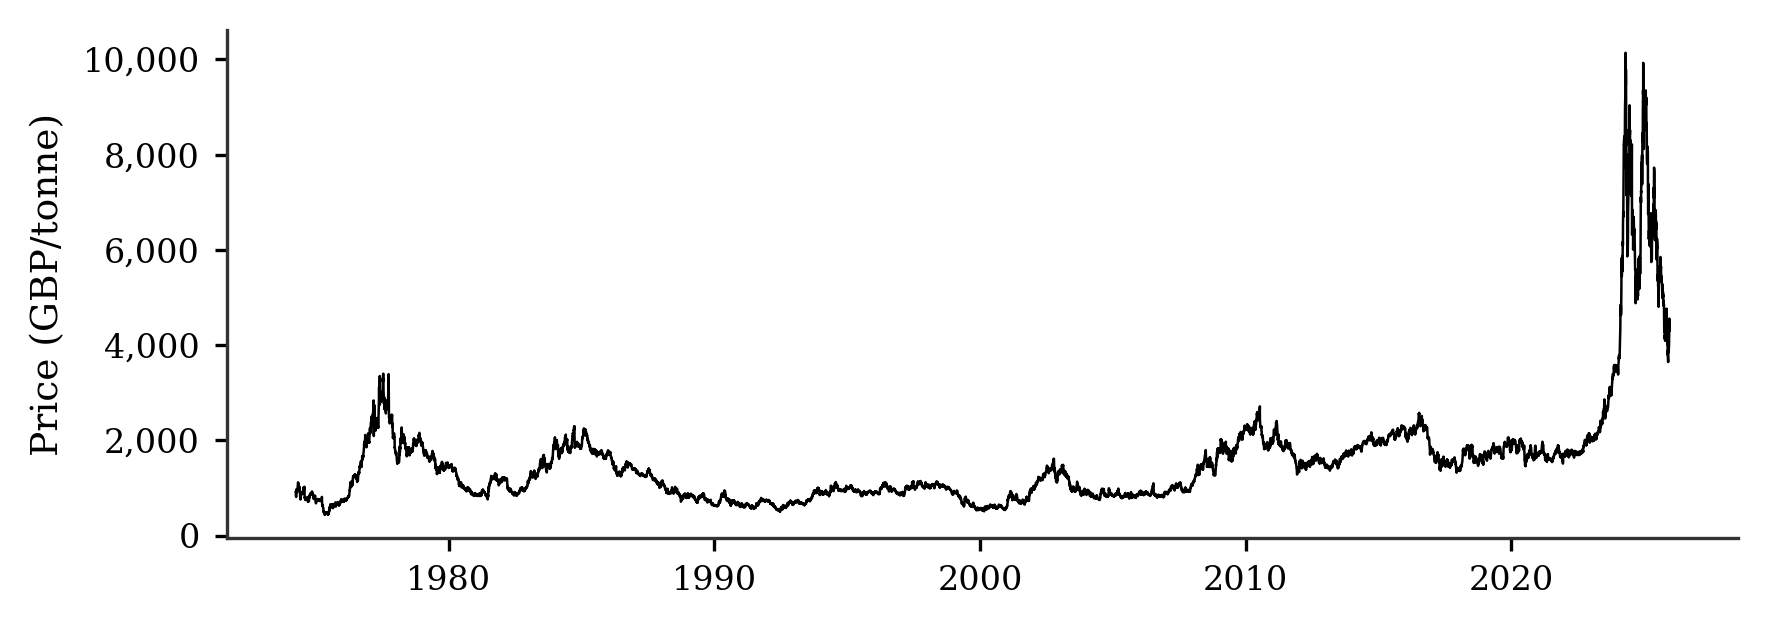
\includegraphics[width=\textwidth]{figures/price_series.png}
\caption{ICE London Cocoa Futures Daily Closing Price (1974--2025)}
\label{fig:price-series}
\begin{tablenotes}
\small
\item \textit{Notes}: Front-month continuous contract (LCCc1) daily closing
prices in GBP per metric tonne. Data source: Refinitiv Workspace.
Sample period: April 1, 1974 -- December 15, 2025 (13,090 trading days).
\end{tablenotes}
\end{figure}

Table~\ref{tab:return-stats} presents descriptive statistics for daily
log-returns. The mean daily return is slightly positive (0.012\%), corresponding
to an approximate annualized mean return of 3\% over the full sample. However,
returns exhibit substantial volatility: the standard deviation of 1.93\%
implies an annualized volatility of approximately 30\%, consistent with cocoa's
classification as a high-volatility commodity. The distribution of returns
deviates sharply from normality. Negative skewness ($-0.997$) indicates a
left tail longer than the right, reflecting the tendency for large negative
price movements to occur more frequently than large positive ones. Excess
kurtosis of 12.96 documents fat tails: extreme returns occur far more often
than a Gaussian distribution would predict. The Jarque-Bera test decisively
rejects normality ($p < 0.001$), confirming that standard volatility models
assuming Gaussian innovations may be misspecified for cocoa returns.

\begin{table}[htbp]
\centering
\caption{Descriptive Statistics for Daily Log-Returns}
\label{tab:return-stats}
\begin{tabular}{lr}
\toprule
\textbf{Statistic} & \textbf{Value} \\
\midrule
Observations & 13,087 \\
Mean (\%) & 0.012 \\
Median (\%) & 0.000 \\
Std. Deviation (\%) & 1.929 \\
Minimum (\%) & $-26.212$ \\
Maximum (\%) & 12.988 \\
25th Percentile (\%) & $-0.917$ \\
75th Percentile (\%) & 0.945 \\
\addlinespace
Skewness & $-0.997$ \\
Excess Kurtosis & 12.963 \\
\addlinespace
Jarque-Bera & 141,013 \\
\quad $p$-value & $<0.001$ \\
\bottomrule
\end{tabular}
\begin{tablenotes}
\small
\item \textit{Notes}: Daily log-returns computed as $r_t = \ln(C_t / C_{t-1})$ for ICE London cocoa front-month continuous contract (LCCc1), April 1974--December 2025. Returns expressed in percentage points. Excess kurtosis reported (normal distribution: 0). Jarque-Bera test strongly rejects normality ($p < 0.001$), consistent with fat tails and negative skewness typical of commodity returns.
\end{tablenotes}
\end{table}


\paragraph{Volatility time series.}
Figure~\ref{fig:volatility-series} displays the Yang-Zhang volatility
estimator (annualized, in percent) computed from daily OHLC data. The
figure reveals pronounced volatility clustering:
periods of high volatility persist for extended intervals before reverting
to lower levels. The late-1970s episode and the 2022--2024 crisis stand out
as the two dominant volatility regimes in the sample. Between these episodes,
volatility fluctuates around a lower baseline with occasional spikes
corresponding to supply shocks, weather events, and financial market
turbulence (e.g., the 2008 financial crisis).

\begin{figure}[htbp]
\centering
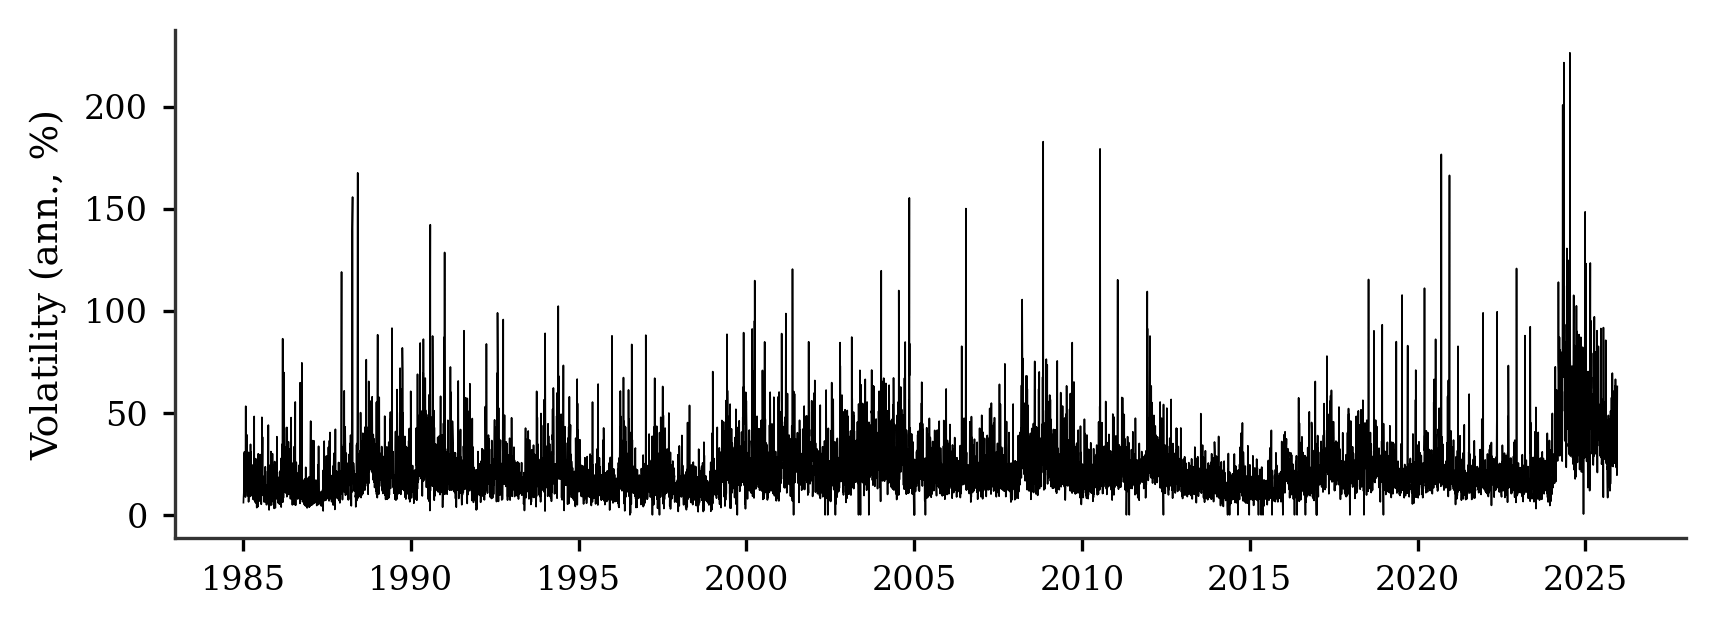
\includegraphics[width=\textwidth]{figures/volatility_timeseries.png}
\caption{Yang-Zhang Annualized Volatility Time Series (1974--2025)}
\label{fig:volatility-series}
\begin{tablenotes}
\small
\item \textit{Notes}: Yang-Zhang volatility estimator computed from daily
OHLC prices and annualized (percent). The estimator combines overnight,
intraday, and close-to-close variance components following
\textcite{yangDriftIndependentVolatility2000}. Pronounced volatility clustering
and regime-switching are evident, motivating the use of HAR models that
capture persistence across multiple horizons.
\end{tablenotes}
\end{figure}

The persistence of volatility justifies the HAR model's multi-horizon
structure: current volatility depends not only on yesterday's volatility
(daily component) but also on average volatility over the past week and
month (weekly and monthly components). The clustering pattern also motivates
quantile regression: during high-volatility regimes, the tails of the
volatility distribution shift outward, and point forecasts of the mean may
underestimate the risk of extreme outcomes.

\paragraph{Stationarity.}
The regression models in Section~\ref{sec:methodology} require stationary
inputs. Table~\ref{tab:stationarity} reports Augmented Dickey--Fuller (ADF)
and Phillips--Perron (PP) unit root tests for the three key series. Both
tests include a constant; ADF lag length is selected by AIC.

\begin{table}[htbp]
\centering
\small
\caption{Unit root tests for stationarity}
\label{tab:stationarity}
\begin{tabular}{lrccrcc}
\toprule
 & & \multicolumn{2}{c}{ADF} & & \multicolumn{2}{c}{PP} \\
\cmidrule(lr){3-4}\cmidrule(lr){6-7}
Series & $N$ & Statistic & $p$-value & & Statistic & $p$-value \\
\midrule
Log returns & 13,087 & $-112.08$ & $<0.001$ & & $-112.09$ & $<0.001$ \\
Yang-Zhang volatility & 13,087 & $-8.42$ & $<0.001$ & & $-90.99$ & $<0.001$ \\
Ni\~no 3.4 anomaly & 787 & $-6.85$ & $<0.001$ & & $-6.46$ & $<0.001$ \\
\bottomrule
\end{tabular}
\par\smallskip
{\footnotesize\textit{Note:} ADF = Augmented Dickey--Fuller test
\parencite{dickey1979distribution}; PP = Phillips--Perron test
\parencite{phillips1988testing}. Both tests include a constant.
ADF lag length selected by AIC. The null hypothesis is a unit root;
rejection indicates stationarity.}
\end{table}

All three series decisively reject the unit root null at the 1\% level.
Log returns are stationary by construction, with ADF and PP statistics
both below $-112$. The Yang-Zhang volatility series exhibits high
persistence---the ADF test requires 39 lags to whiten the residuals---but
remains stationary (ADF $= -8.42$, $p < 0.001$). The large discrepancy
between the ADF and PP statistics ($-8.42$ vs.\ $-90.99$) reflects the
difference in how each test handles serial correlation: ADF augments the
regression with lagged differences, while PP applies a non-parametric
correction to the test statistic. Both agree on rejection. The Ni\~no~3.4
anomaly is stationary by design, as it measures deviations from a
climatological mean, confirmed by both tests (ADF $= -6.85$, PP $= -6.46$,
$p < 0.001$). These results justify the use of standard OLS and quantile
regression methods without differencing or cointegration corrections.

%------------------------------------------------------------------------------

The data described in this section provide the foundation for the empirical
analysis. The extended daily sample (1974--2025) ensures sufficient variation
in both volatility regimes and ENSO phases, while the availability of
intraday data for the recent period enables validation of the Yang-Zhang
volatility proxy. The next section presents the empirical results from the
HAR-based quantile regression models estimated using these data.

\newpage
% Section 5: Results
\section{Empirical Results}
\label{sec:results}

This section presents the out-of-sample forecasting results, organized around
the two research questions. Section~\ref{sec:res-mean} compares mean forecast
accuracy across the three baseline models. Section~\ref{sec:res-har-qr}
evaluates distributional forecasts at the upper tail, testing whether HAR-QR
outperforms the benchmarks across horizons (RQ1). Section~\ref{sec:res-har-x-qr}
assesses whether the Ni\~no~3.4 climate index adds forecast value at long
horizons (RQ2). Section~\ref{sec:res-mcs} tests the statistical significance
of the observed differences using Model Confidence Sets.
Section~\ref{sec:res-summary} synthesizes the findings. All
results use a rolling estimation window of 2,520 trading days with daily
re-estimation, yielding approximately 10,500 out-of-sample
forecast--realization pairs at each horizon.

%------------------------------------------------------------------------------
\subsection{Mean Forecast Comparison}
\label{sec:res-mean}
%------------------------------------------------------------------------------

Table~\ref{tab:mean-qlike} reports the QLIKE loss for the three mean forecast
models across all six horizons. The ranking is unambiguous: HAR-OLS achieves the lowest
(best) QLIKE at every horizon, followed by GARCH(1,1), with historical
volatility uniformly last.

\begin{table}[htbp]
\centering
\small
\caption{Mean forecast QLIKE loss by model and horizon}
\label{tab:mean-qlike}
\begin{tabular}{lcccccc}
\toprule
Model & 1d & 1w & 1m & 3m & 6m & 12m \\
\midrule
Historical Vol    & $-7.002$ & $-7.256$ & $-7.327$ & $-7.334^{*}$ & $-7.324$ & $-7.310$ \\
GARCH(1,1)        & $-7.242$ & $-7.388$ & $-7.406^{*}$ & $-7.381$ & $-7.356$ & $-7.345$ \\
HAR-OLS           & $\mathbf{-7.302}$ & $\mathbf{-7.482}$ & $\mathbf{-7.521}^{*}$ & $\mathbf{-7.515}$ & $\mathbf{-7.492}$ & $\mathbf{-7.485}$ \\
\bottomrule
\end{tabular}
\par\smallskip
{\footnotesize\textit{Note:} QLIKE loss \parencite{pattonVolatilityForecastComparison};
more negative values indicate better forecast performance. Bold: best model
at each horizon. $^{*}$Best horizon for each model.
Evaluation period: approximately 10,500 out-of-sample trading days (1984--2025).}
\end{table}

The gap between HAR-OLS and GARCH is largest at the one-month horizon
(0.115 QLIKE units) and narrowest at one day (0.060 units). This pattern
reflects the structural differences between the two models. GARCH(1,1)
captures short-run volatility dynamics effectively: its conditional
variance process adapts quickly to recent shocks. But its exponential
memory decay means that multi-step forecasts converge rapidly toward the
unconditional variance, erasing the model's informational advantage at
longer horizons. HAR-OLS, by contrast, includes a monthly volatility
component ($\sigma^{(m)}_t$) that captures persistence at lower
frequencies. This component maintains a correlation of 0.66 with the
twelve-month target, compared to 0.37 for the daily component, explaining
why HAR-OLS retains a substantial edge even at twelve months.

Historical volatility performs worst because it is the most constrained:
its trailing average cannot distinguish between a volatility spike driven
by a transient shock and a persistent regime change. Nevertheless, all
three models share a common horizon pattern: loss improves from the
one-day to the one-month horizon, reflecting the smoothing effect of
averaging in the target $\bar{\sigma}_{t:t+h}$, before degrading at
six and twelve months as the autoregressive signal weakens. The fact
that even HAR-OLS degrades beyond one month confirms the fundamental
difficulty of long-horizon volatility forecasting and motivates the
search for additional predictive signals in Section~\ref{sec:res-har-x-qr}.

The QLIKE ranking is confirmed by MSE and MAE. Figure~\ref{fig:robustness-lineplot}
plots all three loss functions across horizons. HAR-OLS achieves the lowest
MSE at every horizon; MAE is minimized by HAR-X-QR (median) at short horizons
and by HAR-OLS or HAR-QR (median) beyond three months. Crucially, GARCH(1,1)
is the worst-performing model under all three metrics at long horizons,
with its error rising steeply relative to the HAR family as the horizon
extends, a direct consequence of mean-reversion in its multi-step forecasts.
The HAR family dominates regardless of how point forecast errors are penalized.

\begin{figure}[htbp]
\centering

\includegraphics[width=0.92\textwidth]{figures/robustness_metrics_lineplot.pdf}
\caption{Robustness check: point forecast accuracy under three loss functions}
\label{fig:robustness-lineplot}
{\footnotesize\textit{Notes}: Each panel plots mean (or median) forecast loss
across horizons. QLIKE axis is inverted (more negative = better). MSE scaled
by $10^5$ for readability. All models evaluated on the same out-of-sample
period. The consistent separation between GARCH(1,1) and the HAR family at
long horizons holds across all three metrics.}
\end{figure}

%------------------------------------------------------------------------------
\subsection{Quantile Forecast Comparison (RQ1)}
\label{sec:res-har-qr}
%------------------------------------------------------------------------------

Mean forecasts summarize only the center of the conditional distribution.
For risk assessment, the upper tail matters: a model that accurately forecasts
average volatility may still understate the probability of extreme outcomes.
We now compare five models on their ability to forecast the 95th percentile
of future volatility. Historical volatility uses the empirical quantile of
the trailing 252-day distribution. GARCH(1,1) quantiles follow the
closed-form Gaussian approach (Equation~\ref{eq:garch-quantile}). HAR-OLS
produces pseudo-quantile forecasts from its in-sample residual distribution
(Equation~\ref{eq:har-ols-quantile}). HAR-QR estimates the quantile directly
through quantile regression on the HAR structure, and HAR-X-QR augments
this with the Ni\~no~3.4 index.

Table~\ref{tab:upper-qlike-comparison} reports the quantile loss at
$\tau = 0.95$ for all five models. Figure~\ref{fig:ql95-comparison}
presents the same comparison graphically.

\begin{table}[htbp]
\centering
\small
\caption{Upper-tail quantile loss ($\tau = 0.95$) by model and horizon}
\label{tab:upper-qlike-comparison}
\begin{tabular}{lcccccc}
\toprule
Model & 1d & 1w & 1m & 3m & 6m & 12m \\
\midrule
Historical Vol    & $0.001502$ & $0.001023$ & $0.000871^{*}$ & $0.000889$ & $0.000914$ & $0.000930$ \\
GARCH(1,1)        & $0.001393$ & $0.001067$ & $0.001011^{*}$ & $0.001053$ & $0.001066$ & $0.001044$ \\
HAR-OLS           & $0.001272$ & $0.000748$ & $0.000507$ & $0.000472$ & $0.000479$ & $0.000451^{*}$ \\
HAR-QR            & $\mathbf{0.001193}$ & $\mathbf{0.000692}$ & $\mathbf{0.000458}$ & $0.000433^{*}$ & $0.000454$ & $0.000446$ \\
HAR-X-QR          & $0.001195$ & $0.000695$ & $0.000464$ & $\mathbf{0.000418}$ & $\mathbf{0.000387}$ & $\mathbf{0.000333}^{*}$ \\
\bottomrule
\end{tabular}
\par\smallskip
{\footnotesize\textit{Note:} Quantile loss as defined in
Equation~\eqref{eq:quantile-loss}. Lower values indicate better forecasts.
Bold: best model at each horizon. $^{*}$Best horizon for each model.
Historical Vol quantiles are empirical percentiles of the
trailing 252-day volatility distribution. GARCH quantiles use the
closed-form Gaussian approach (Equation~\ref{eq:garch-quantile}).
HAR-OLS quantiles are pseudo-quantile forecasts from in-sample
residuals (Equation~\ref{eq:har-ols-quantile}).}
\end{table}

\begin{figure}[htbp]
\centering

\includegraphics[width=\textwidth]{figures/ql95_comparison.png}
\caption{Upper-tail quantile loss ($\tau = 0.95$) across forecast horizons}
\label{fig:ql95-comparison}
\begin{tablenotes}
\small
\item \textit{Notes}: Lower values indicate better upper-tail forecasts.
The HAR family (HAR-OLS, HAR-QR, HAR-X-QR) dominates both non-parametric
and GARCH benchmarks at all horizons. HAR-X-QR (ENSO-augmented) separates
from HAR-QR at horizons beyond three months.
The y-axis starts at zero for honest visual comparison.
\end{tablenotes}
\end{figure}

Four patterns emerge from this comparison.

\textit{First, the HAR family dominates all benchmarks at every horizon.}
HAR-QR, HAR-OLS, and HAR-X-QR all outperform both GARCH(1,1) and
historical volatility at every horizon. The gap is not marginal: at twelve
months, the best benchmark (historical volatility, $0.000930$) is 108\%
above HAR-QR ($0.000446$) and 179\% above HAR-X-QR ($0.000333$). The HAR
structure---which conditions on heterogeneous volatility lags at daily,
weekly, and monthly frequencies---captures distributional persistence that
neither the rolling unconditional distribution (historical volatility) nor
the parametric GARCH model can exploit at procurement-relevant horizons.

\textit{Second, direct quantile estimation outperforms the pseudo-quantile
approach.} HAR-QR beats the HAR-OLS pseudo-quantile at every horizon,
with improvements of 6\% at one day ($0.001193$ vs $0.001272$), 10\% at
one month ($0.000458$ vs $0.000507$), and 1\% at twelve months ($0.000446$
vs $0.000451$). The gap is widest at short-to-medium horizons, where
volatility dynamics are more state-dependent and the conditional quantile
diverges from the unconditional residual distribution. At twelve months,
the near-convergence of the two HAR variants indicates that the HAR
regressors themselves carry most of the distributional information at very
long horizons; the marginal contribution of re-weighting via quantile
regression is modest once the ENSO regressor is absent. This confirms
that the HAR-OLS pseudo-quantile is a useful benchmark: the advantage of
explicit quantile regression is real but bounded.

\textit{Third, GARCH's Gaussian closed-form systematically underestimates
extreme volatility beyond the short horizon.} At one day, GARCH ($0.001393$)
outperforms historical volatility ($0.001502$), reflecting the GARCH
model's ability to condition the forecast distribution on the current
volatility state. From one week onward, however, GARCH's Gaussian
quantile assumption deteriorates. The closed-form formula uses the
in-sample standard deviation of Yang-Zhang volatility as forecast
uncertainty (Equation~\ref{eq:garch-quantile}), which is a static measure
that cannot adapt to the non-Gaussian, right-skewed shape of the
volatility distribution at longer horizons. GARCH consequently places the
$\tau = 0.95$ boundary too low, leading to excess violations and the
highest quantile loss of all five models from one week onward. By twelve
months, GARCH's quantile loss ($0.001044$) is 134\% above HAR-QR's
($0.000446$).

\textit{Fourth, HAR-X-QR separates from HAR-QR only at long horizons.}
At one day through one month, the two HAR-QR models are virtually
indistinguishable (differences $<3\%$). The divergence begins at three
months ($+3.26\%$ improvement) and accelerates to $+14.66\%$ at six months
and $+25.44\%$ at twelve months. This horizon dependence is analyzed in
detail in Section~\ref{sec:res-har-x-qr}.

These findings answer RQ1: the HAR-QR model forecasts the upper tail of
the conditional volatility distribution more accurately than all three
benchmarks (historical volatility, GARCH(1,1), and HAR-OLS pseudoquantile)
at all horizons from one day to twelve months.

Figures~\ref{fig:upper-tail-1m} and~\ref{fig:upper-tail-12m} illustrate
this comparison visually. Each figure overlays the $\tau = 0.95$ forecast
boundary from all four models on realized volatility for the 2015--2025
window, which includes the 2022--2024 cocoa supply crisis.

At the one-month horizon (Figure~\ref{fig:upper-tail-1m}), the HAR-QR
and HAR-X-QR boundaries track the realized upper tail closely, rising
in tandem with the crisis spike. GARCH's boundary reacts with a visible
lag, and historical volatility's boundary is the slowest to adjust. At
the twelve-month horizon (Figure~\ref{fig:upper-tail-12m}), the
differences are more pronounced: the HAR-X-QR boundary rises ahead of
the crisis period, reflecting the ENSO regressor's contribution, while
the GARCH boundary remains comparatively flat, a direct consequence of
its mean-reverting multi-step forecasts converging toward the
unconditional variance.

\begin{figure}[htbp]
\centering
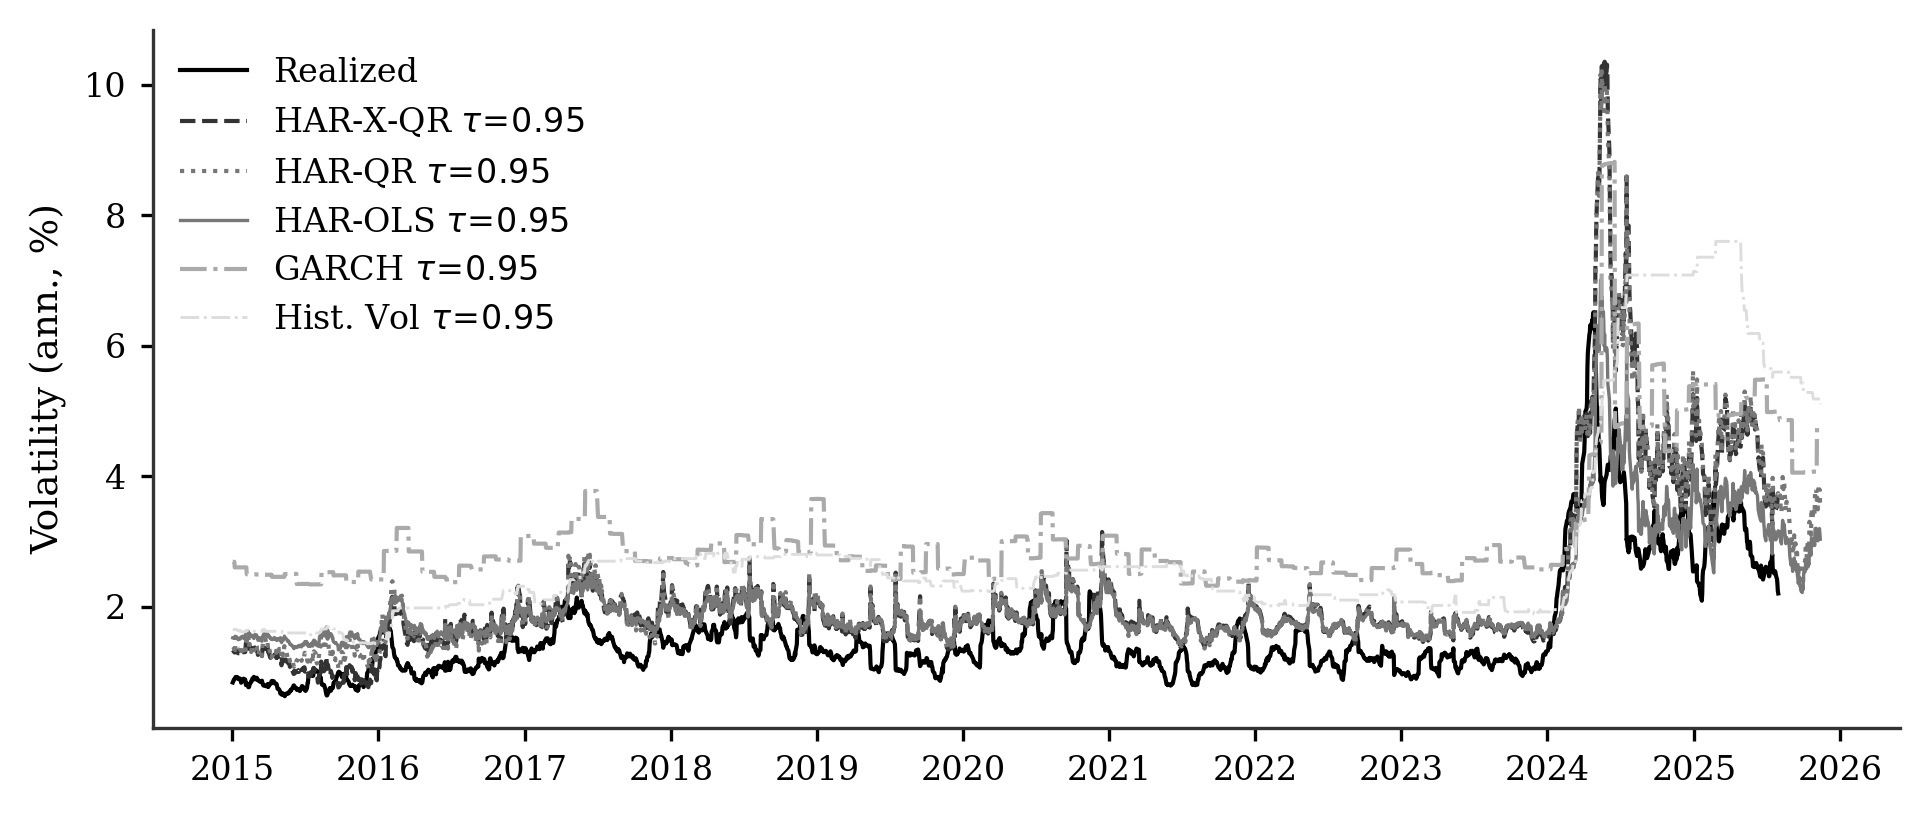
\includegraphics[width=\textwidth]{figures/upper_tail_1m.png}
\caption{Upper-tail ($\tau = 0.95$) forecast comparison at the one-month horizon}
\label{fig:upper-tail-1m}
\begin{tablenotes}
\small
\item \textit{Notes}: Realized Yang-Zhang volatility (solid black) and
$\tau = 0.95$ quantile forecasts from the five models. Zoomed to 2015--2025
to show the 2022--2024 supply crisis period in detail.
\end{tablenotes}
\end{figure}

\begin{figure}[htbp]
\centering
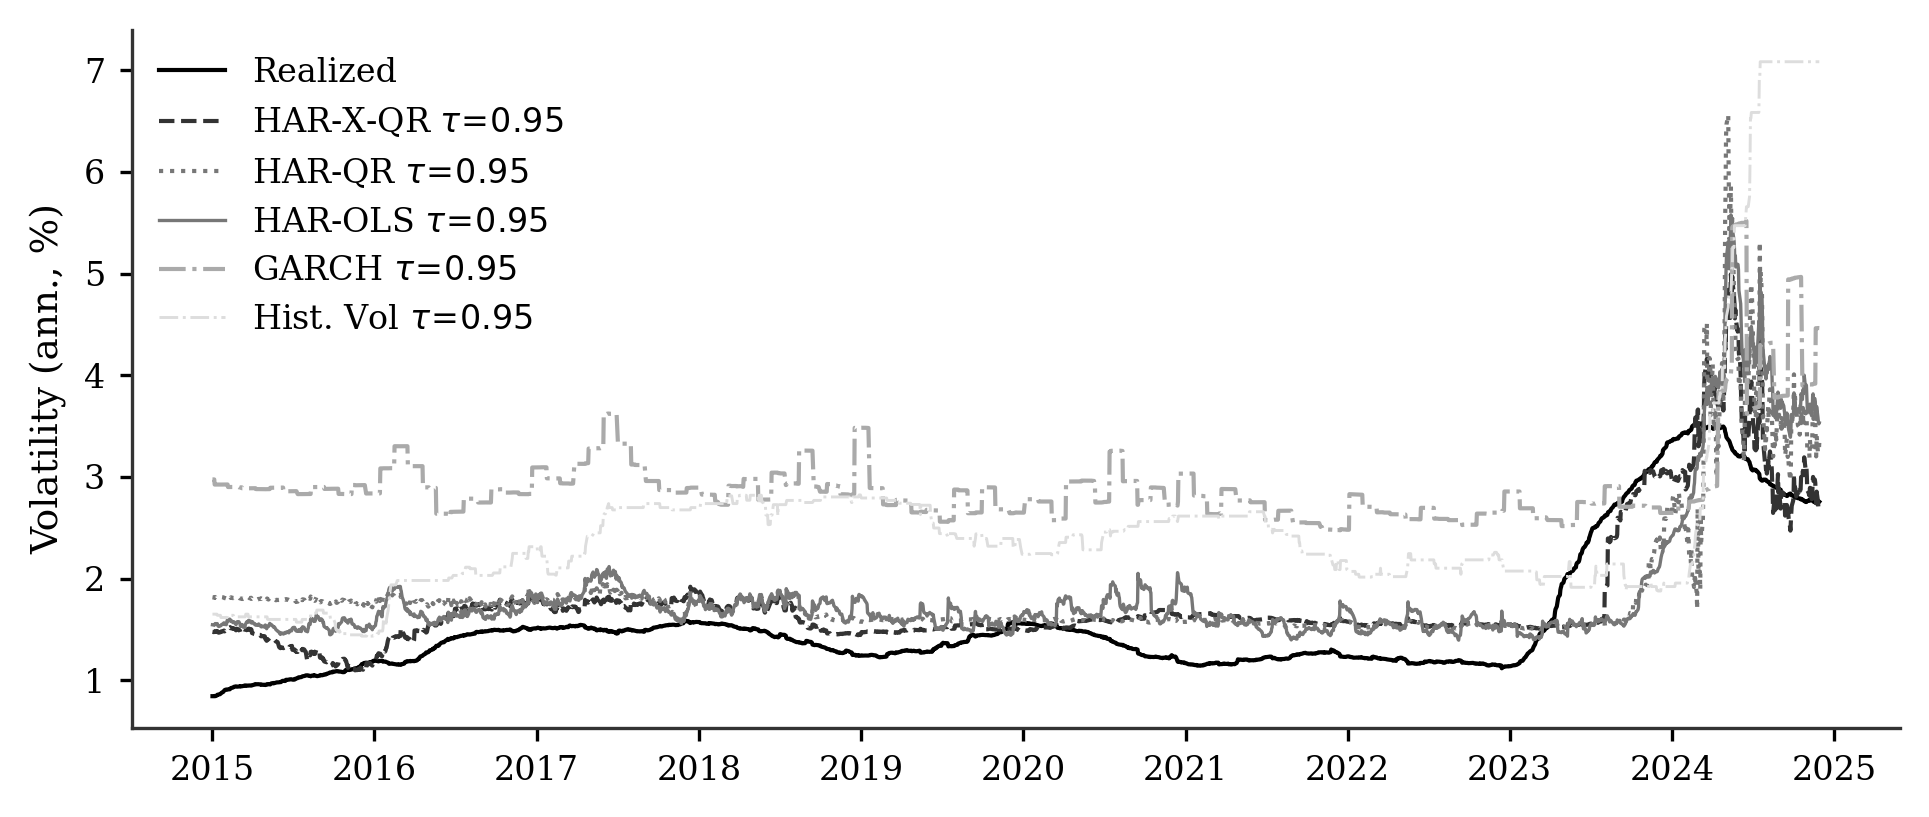
\includegraphics[width=\textwidth]{figures/upper_tail_12m.png}
\caption{Upper-tail ($\tau = 0.95$) forecast comparison at the twelve-month horizon}
\label{fig:upper-tail-12m}
\begin{tablenotes}
\small
\item \textit{Notes}: Same construction as Figure~\ref{fig:upper-tail-1m}.
At the twelve-month horizon, HAR-X-QR's boundary rises ahead of the
crisis period, while GARCH's boundary remains comparatively flat due to
mean-reversion in its multi-step variance forecast and the Gaussian
tail assumption.
\end{tablenotes}
\end{figure}

Table~\ref{tab:har-qr-coverage} reports violation rates for the
HAR-QR upper quantile ($\tau = 0.95$) by horizon. Under correct
conditional coverage, the violation rate should equal $1 - \tau = 5\%$.
At the one-day and one-week horizons, the model achieves near-target
coverage (4.84\% and 5.15\%). Coverage remains acceptable through
the three-month horizon (5.90\%), but exceeds the target at six months
(7.04\%) and twelve months (8.34\%). The coverage degradation at long
horizons indicates that the autoregressive signal alone becomes
insufficient to track extreme upper-tail volatility: the HAR
structure, while dominant among the models tested, still
underestimates how far the distribution can shift in periods of
sustained supply stress. This motivates the ENSO augmentation
examined next.

\begin{table}[htbp]
\centering
\small
\caption{HAR-QR upper-quantile ($\tau = 0.95$) coverage by horizon}
\label{tab:har-qr-coverage}
\begin{tabular}{lrrr}
\toprule
Horizon & $N$ & Violations & Violation rate (\%) \\
\midrule
1d  & 10,545 & 510 & 4.84 \\
1w  & 10,541 & 543 & 5.15 \\
1m  & 10,524 & 600 & 5.70 \\
3m  & 10,480 & 618 & 5.90 \\
6m  & 10,414 & 733 & 7.04 \\
12m & 10,282 & 857 & 8.34 \\
\bottomrule
\end{tabular}
\par\smallskip
{\footnotesize\textit{Note:} A violation occurs when realized volatility
exceeds the $\tau = 0.95$ quantile forecast. Under correct specification,
the violation rate should equal 5\%. $N$ denotes the number of
forecast--realization pairs at each horizon.}
\end{table}

%------------------------------------------------------------------------------
\subsection{ENSO Augmentation: HAR-X-QR (RQ2)}
\label{sec:res-har-x-qr}
%------------------------------------------------------------------------------

Table~\ref{tab:har-x-improvement} reports the percentage change in quantile
loss when moving from HAR-QR to HAR-X-QR across all three quantile levels
and six horizons. Positive values indicate improvement (lower loss under
HAR-X-QR).

\begin{table}[htbp]
\centering
\small
\caption{Quantile loss improvement (\%) from ENSO augmentation (HAR-X-QR
vs.\ HAR-QR)}
\label{tab:har-x-improvement}
\begin{tabular}{lrrrrrr}
\toprule
$\tau$ & 1d & 1w & 1m & 3m & 6m & 12m \\
\midrule
0.50 & $-0.0076$ & $-0.2093$ & $-0.2698$ & $-0.3994$ & $-0.0643$ & $+1.1225$ \\
0.75 & $-0.0357$ & $-0.1810$ & $-0.6684$ & $-1.3689$ & $-0.5717$ & $-0.8660$ \\
0.95 & $-0.1628$ & $-0.5111$ & $-1.4628$ & $+3.2564$ & $+14.6602$ & $+25.4375$ \\
\bottomrule
\end{tabular}
\par\smallskip
{\footnotesize\textit{Note:} Positive values indicate that HAR-X-QR achieves
lower quantile loss than HAR-QR. Computed as $(1 -
\text{QL}_{\text{HAR-X}} / \text{QL}_{\text{HAR}}) \times 100$.}
\end{table}

The results reveal a striking horizon- and quantile-dependent pattern.
At short horizons (one day to one month), ENSO augmentation provides no
benefit and occasionally worsens forecasts marginally. At such horizons,
the Ni\~no~3.4 coefficient captures noise rather than signal, and the
additional parameter slightly degrades out-of-sample performance.

The first meaningful improvement appears at three months for the upper
tail: $\tau = 0.95$ quantile loss decreases by 3.26\%. The effect
strengthens substantially at six months ($+14.66\%$) and reaches its
maximum at twelve months ($+25.44\%$). This concentration in the upper
tail is consistent with the hypothesis that ENSO anomalies are associated
with cocoa supply disruptions, which manifest as rightward shifts in the
volatility distribution rather than a uniform upward shift. Whether this
recalibration reflects a stable predictive relationship or a sample-specific
regime effect is assessed in Section~\ref{sec:res-robustness}. The GARCH and
historical volatility benchmarks cannot exploit this climate index, explaining
why their twelve-month upper-tail performance in
Table~\ref{tab:upper-qlike-comparison} falls far behind HAR-X-QR:
historical volatility's loss ($0.000930$) is 179\% higher than
HAR-X-QR's ($0.000333$), and GARCH's ($0.001044$) is 213\% higher.

The median ($\tau = 0.50$) shows only modest improvement
($+1.12\%$), confirming that the benefit of ENSO augmentation is
predominantly distributional rather than centered on the mean.

Table~\ref{tab:coverage-comparison} examines how ENSO augmentation
affects upper-tail ($\tau = 0.95$) coverage calibration. HAR-X-QR achieves
substantially lower quantile loss but its violation rate at twelve months
rises to 10.29\%, compared to 8.34\% under HAR-QR. These two facts are
not contradictory: they reflect the asymmetric check function and how the
ENSO coefficient recalibrates the forecast boundary across climate regimes.
At $\tau = 0.95$, the positive ENSO coefficient raises the boundary during
El~Ni\~no episodes and lowers it when the Ni\~no~3.4 anomaly is negative
(La~Ni\~na). The lower boundary during La~Ni\~na conditions is breached
more often when unexpected shocks occur, raising the overall violation
rate. The quantile loss gain comes from El~Ni\~no episodes: when realized
volatility spikes severely, the elevated boundary reduces the magnitude
of exceedances substantially. The asymmetric check function penalizes
large under-predictions more heavily than over-predictions, so the
large-episode reductions outweigh the additional La~Ni\~na-period breaches
in average loss. The net result is a model that is better calibrated
\emph{when it matters most} (large upside events) but less well calibrated
overall.

\begin{table}[htbp]
\centering
\small
\caption{Coverage comparison: violation rates (\%) for HAR-QR and HAR-X-QR}
\label{tab:coverage-comparison}
\begin{tabular}{lrr}
\toprule
 & \multicolumn{2}{c}{Upper tail ($\tau = 0.95$)} \\
\cmidrule(lr){2-3}
Horizon & HAR-QR & HAR-X-QR \\
\midrule
1d  & 4.84 & 4.80 \\
1w  & 5.15 & 5.22 \\
1m  & 5.68 & 6.13 \\
3m  & 5.91 & 6.49 \\
6m  & 7.04 & 8.91 \\
12m & 8.34 & 10.29 \\
\bottomrule
\end{tabular}
\par\smallskip
{\footnotesize\textit{Note:} Under correct specification, the violation
rate should equal 5\%. Values closer to 5\% indicate better calibration.
$N \approx 10{,}400$--$10{,}500$ forecast--realization pairs per horizon.}
\end{table}

%------------------------------------------------------------------------------
\subsection{Statistical Significance: Model Confidence Sets}
\label{sec:res-mcs}
%------------------------------------------------------------------------------

The preceding sections compare models by point estimates of loss functions.
To assess whether the observed differences are statistically significant,
we apply the Model Confidence Set (MCS) procedure of
\textcite{hansen2011model}. The MCS identifies the set
$\mathcal{M}^{*}$ of models whose forecasting ability cannot be
distinguished from that of the best model at a given confidence level.
We use the MCS procedure and configuration described in
Section~\ref{sec:meth-evaluation}.

Table~\ref{tab:mcs-qlike} reports MCS results for QLIKE loss.
HAR-OLS is the sole member of $\mathcal{M}^{*}$ at the one-day
and one-week horizons ($p = 1.00$), confirming that its mean forecast
superiority over GARCH and historical volatility is statistically
significant at short horizons. From one month onward, the HAR-QR
and HAR-X-QR median forecasts enter $\mathcal{M}^{*}$, indicating
that their mean forecast accuracy is statistically indistinguishable
from HAR-OLS at longer horizons. GARCH(1,1) is excluded from
$\mathcal{M}^{*}$ at every horizon; its inferior QLIKE performance
is not attributable to sampling variation.

\begin{table}[htbp]
\centering
\small
\caption{Model Confidence Set: QLIKE loss (mean forecasts)}
\label{tab:mcs-qlike}
\begin{tabular}{lccccccc}
\toprule
 & & \multicolumn{6}{c}{Horizon} \\
\cmidrule(lr){3-8}
Model & & 1d & 1w & 1m & 3m & 6m & 12m \\
\midrule
Historical Vol    & $p$ & 0.01 & 0.04 & 0.07 & 0.10 & 0.10 & 0.06 \\
                  & $\mathcal{M}^{*}$ &  &  &  &  & $\checkmark$ &  \\
\addlinespace
GARCH(1,1)        & $p$ & 0.01 & 0.00 & 0.00 & 0.00 & 0.00 & 0.01 \\
                  & $\mathcal{M}^{*}$ &  &  &  &  &  &  \\
\addlinespace
HAR-OLS           & $p$ & $\mathbf{1.00}$ & $\mathbf{1.00}$ & $\mathbf{1.00}$ & $\mathbf{1.00}$ & $\mathbf{1.00}$ & $\mathbf{1.00}$ \\
                  & $\mathcal{M}^{*}$ & $\checkmark$ & $\checkmark$ & $\checkmark$ & $\checkmark$ & $\checkmark$ & $\checkmark$ \\
\addlinespace
HAR-QR (med.)     & $p$ & 0.00 & 0.04 & 0.10 & 0.38 & 0.30 & 0.25 \\
                  & $\mathcal{M}^{*}$ &  &  & $\checkmark$ & $\checkmark$ & $\checkmark$ & $\checkmark$ \\
\addlinespace
HAR-X-QR (med.)   & $p$ & 0.00 & 0.04 & 0.10 & 0.31 & 0.30 & 0.25 \\
                  & $\mathcal{M}^{*}$ &  &  & $\checkmark$ & $\checkmark$ & $\checkmark$ & $\checkmark$ \\
\bottomrule
\end{tabular}
\par\smallskip
{\footnotesize\textit{Note:} MCS $p$-values from \textcite{hansen2011model};
max-$t$ statistic, 10,000 stationary bootstrap replications, 90\%
confidence level. $\checkmark$ indicates membership in
$\mathcal{M}^{*}$. Bold: $p = 1.00$ (best model). HAR-QR and
HAR-X-QR evaluated on their median ($\tau = 0.50$) forecasts.}
\end{table}

Table~\ref{tab:mcs-ql95} presents MCS results for quantile loss at
$\tau = 0.95$, the central evaluation criterion for distributional
forecasting. Historical volatility and GARCH(1,1) are excluded from
$\mathcal{M}^{*}$ at every horizon ($p < 0.05$ throughout), confirming
that their inferior quantile loss is statistically significant and not
a product of sampling variation. From one month onward, $\mathcal{M}^{*}$
contains HAR-OLS alongside the two direct quantile regression models,
indicating that the pseudo-quantile approach is statistically
indistinguishable from HAR-QR at medium and long horizons. At short
horizons, however, HAR-OLS is excluded ($p = 0.04$ at one day,
$p = 0.02$ at one week), confirming that explicit quantile estimation
provides a statistically significant advantage where volatility dynamics
are most state-dependent.

Within the HAR family, a revealing pattern emerges. At the one-day
horizon, HAR-QR is the sole member of $\mathcal{M}^{*}$ ($p = 1.00$),
with HAR-X-QR narrowly excluded ($p = 0.05$). From one week onward,
both models coexist in $\mathcal{M}^{*}$. The critical shift occurs at
three months: HAR-X-QR takes $p = 1.00$ from HAR-QR, indicating that
the ENSO-augmented model becomes the top-ranked specification. This
reversal persists at six and twelve months ($p = 1.00$ for HAR-X-QR
versus $p = 0.18$ and $p = 0.19$ for HAR-QR). Both models remain in
$\mathcal{M}^{*}$ throughout, meaning the data do not permit a
statistically significant ranking between them. The consistent shift of
the top rank to HAR-X-QR from three months onward is descriptively
suggestive, but any interpretation as evidence for a structural ENSO
channel requires the robustness assessment in
Section~\ref{sec:res-robustness}.

\begin{table}[htbp]
\centering
\small
\caption{Model Confidence Set: quantile loss at $\tau = 0.95$}
\label{tab:mcs-ql95}
\begin{tabular}{lccccccc}
\toprule
 & & \multicolumn{6}{c}{Horizon} \\
\cmidrule(lr){3-8}
Model & & 1d & 1w & 1m & 3m & 6m & 12m \\
\midrule
Historical Vol    & $p$ & 0.04 & 0.00 & 0.00 & 0.00 & 0.00 & 0.00 \\
                  & $\mathcal{M}^{*}$ &  &  &  &  &  &  \\
\addlinespace
GARCH(1,1)        & $p$ & 0.00 & 0.00 & 0.00 & 0.00 & 0.00 & 0.00 \\
                  & $\mathcal{M}^{*}$ &  &  &  &  &  &  \\
\addlinespace
HAR-OLS           & $p$ & 0.04 & 0.02 & 0.17 & 0.23 & 0.17 & 0.15 \\
                  & $\mathcal{M}^{*}$ &  &  & $\checkmark$ & $\checkmark$ & $\checkmark$ & $\checkmark$ \\
\addlinespace
HAR-QR            & $p$ & $\mathbf{1.00}$ & $\mathbf{1.00}$ & $\mathbf{1.00}$ & 0.50 & 0.18 & 0.20 \\
                  & $\mathcal{M}^{*}$ & $\checkmark$ & $\checkmark$ & $\checkmark$ & $\checkmark$ & $\checkmark$ & $\checkmark$ \\
\addlinespace
HAR-X-QR          & $p$ & 0.05 & 0.19 & 0.37 & $\mathbf{1.00}$ & $\mathbf{1.00}$ & $\mathbf{1.00}$ \\
                  & $\mathcal{M}^{*}$ &  & $\checkmark$ & $\checkmark$ & $\checkmark$ & $\checkmark$ & $\checkmark$ \\
\bottomrule
\end{tabular}
\par\smallskip
{\footnotesize\textit{Note:} Same MCS configuration as
Table~\ref{tab:mcs-qlike}. $\checkmark$ indicates membership in
$\mathcal{M}^{*}$ at the 90\% confidence level. Bold: $p = 1.00$
(best model). HAR-OLS pseudo-quantile forecasts are included alongside
the direct quantile models. The shift of $p = 1.00$ from HAR-QR to
HAR-X-QR at three months reflects the onset of HAR-X-QR's ranking
advantage in the evaluation sample.}
\end{table}

%------------------------------------------------------------------------------
\subsection{Robustness of the ENSO Signal}
\label{sec:res-robustness}
%------------------------------------------------------------------------------

The preceding results establish that HAR-X-QR outperforms HAR-QR over the
full evaluation sample, particularly at the twelve-month upper tail. Before interpreting this as evidence
of a structural ENSO--cocoa volatility channel, we apply the three robustness
diagnostics outlined in Section~\ref{sec:methodology}: temporal stability, lag
structure, and cross-commodity replication. Each addresses a distinct way in
which the full-sample gain could be sample-specific rather than generalisable.

\subsubsection*{Temporal stability: expanding-window diagnostic}

To assess whether the ENSO gain is concentrated in the 2022--2024 supply
crisis, we trace the \emph{cumulative} gain as the evaluation horizon
advances through time. For each calendar month~$T$ in the out-of-sample
period, define
\[
\Delta\text{QL}(T) \;=\;
  \text{QL}_{\text{HAR-X-QR}}\!\bigl(\{t \leq T\}\bigr)
  \;-\;
  \text{QL}_{\text{HAR-QR}}\!\bigl(\{t \leq T\}\bigr),
\]
where each loss is computed over all forecast--realisation pairs with
evaluation date up to and including~$T$. Negative values indicate that ENSO
augmentation has been beneficial on a cumulative basis up to that point. The
construction is fully recursive: no break date is assumed or imposed, and
the curve spans the complete out-of-sample window without any
ex-post partitioning.

\begin{figure}[htbp]
\centering
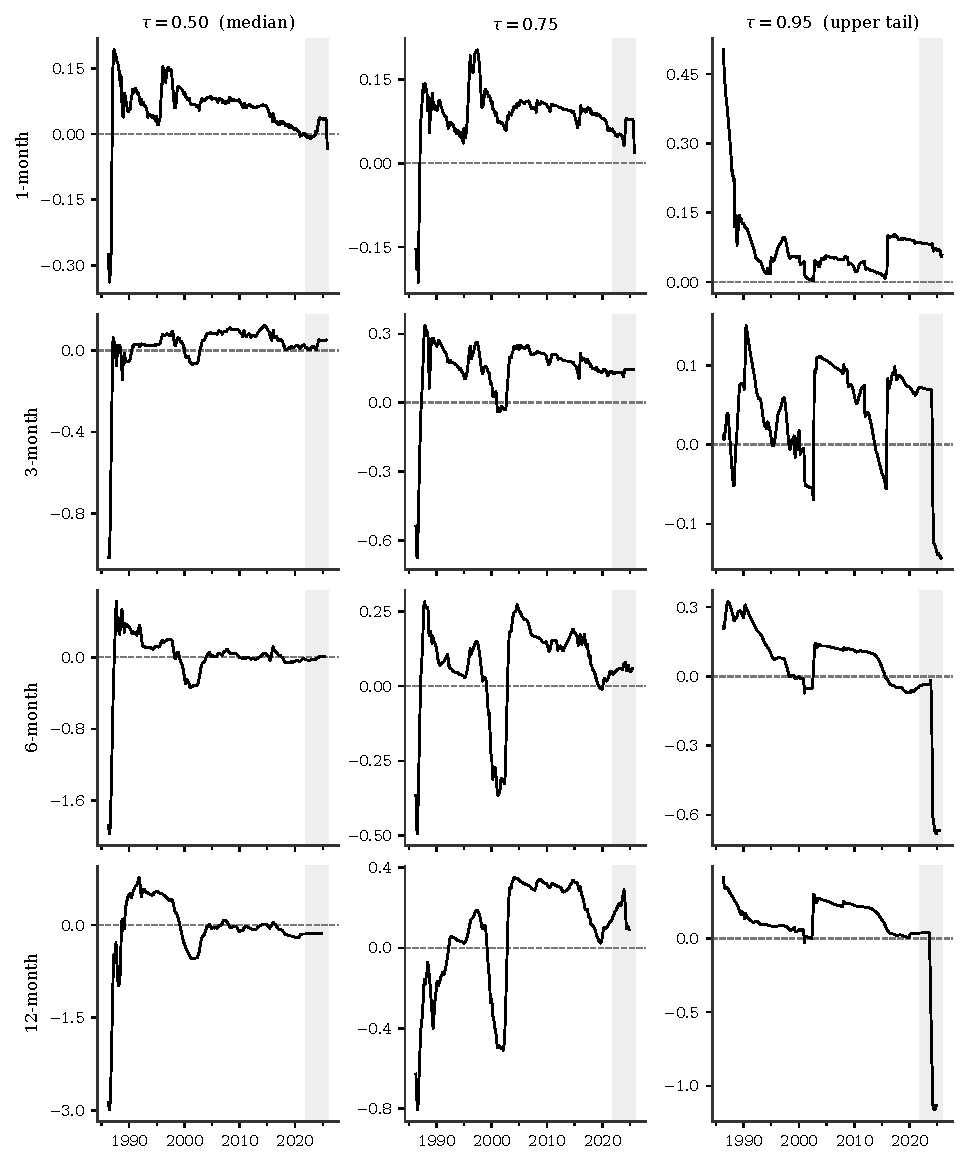
\includegraphics[width=\textwidth]{figures/37_expanding_window_enso_matrix.pdf}
\caption{Expanding-window cumulative ENSO augmentation gain ($\Delta$QL)
  across horizons and quantile levels}
\label{fig:expanding-enso}
{\footnotesize\textit{Notes:} Each panel shows $\Delta\text{QL}(T)$ computed
over all out-of-sample pairs with evaluation date $\leq T$. Negative values
indicate cumulative net gain from ENSO augmentation. Rows: forecast
horizons (1, 3, 6, 12~months). Columns: quantile levels
$\tau \in \{0.50,\, 0.75,\, 0.95\}$. Shaded region marks the post-2022
supply-crisis episode for orientation; no formal cutoff is assumed.
Minimum 500 observations before plotting.}
\end{figure}

Figure~\ref{fig:expanding-enso} shows that the full-sample ENSO gain is
almost entirely a product of the 2022--2024 extreme-volatility episode,
and that this concentration is specific to the upper tail.

At the twelve-month horizon and $\tau = 0.95$, the cumulative $\Delta$QL
remains positive (ENSO augmentation harmful on net) or indistinguishable
from zero throughout the period prior to 2022. The curve then falls sharply
during 2023 and 2024, with the entire full-sample improvement of $25.4\%$
accumulating within those two years. At the six-month horizon the pattern
is similar: a modest negative signal builds gradually from around 2014,
but the dominant movement occurs in the 2023--2024 window, when the
six-month curve falls from near zero to its full-sample endpoint of
$\Delta\text{QL} = -0.67 \times 10^{-4}$.

The median ($\tau = 0.50$) and $\tau = 0.75$ columns tell a qualitatively
different story. Across all four horizons those panels show irregular,
oscillating paths that cross zero repeatedly and never accumulate a
sustained downward trend, even during the 2022--2024 crisis window. The
ENSO augmentation gain is therefore not a broad distributional shift but a
recalibration concentrated in the extreme upper tail. This is consistent
with the mechanism described in Section~\ref{sec:res-har-x-qr}: the
positive ENSO coefficient raises the $\tau = 0.95$ boundary during
El~Ni\~no episodes, reducing the magnitude of large upside exceedances,
while leaving the center of the distribution largely unaffected.

This result sharpens the robustness assessment. The expanding-window
diagnostic shows \emph{when} the gain first accumulates and \emph{where}
in the distribution it is concentrated. For the twelve-month upper tail,
the answer to both questions is the same: almost exclusively during the
2022--2024 supply crisis. The reported $25.4\%$ full-sample improvement
reflects a gain that accrued in the final two years of the evaluation
period and is absent from the median and $\tau = 0.75$ forecasts throughout.

\subsubsection*{Lag structure}

If ENSO drives cocoa volatility through the agronomic-transmission chain
(ENSO anomaly $\to$ West African rainfall $\to$ growing-season disruption $\to$
harvest shortfall $\to$ supply tightening $\to$ price volatility), the
predictive power of the Ni\~no~3.4 index should \emph{strengthen} as the lag
approaches 6--12 months, the time over which this chain unfolds. To test this,
Table~\ref{tab:lag-decay} reports quantile loss at $\tau = 0.95$ for HAR-X-QR
with ENSO lagged 0, 1, 3, and 6 months.

\begin{table}[htbp]
\centering
\small
\caption{Lag-decay diagnostic: quantile loss ($\tau = 0.95$) by ENSO lag}
\label{tab:lag-decay}
\begin{tabular}{lcccc}
\toprule
 & \multicolumn{4}{c}{ENSO lag (months)} \\
\cmidrule(lr){2-5}
Horizon & 0 & 1 & 3 & 6 \\
\midrule
1m  & $0.000464$ & $0.000461$ & $0.000456$ & $0.000457$ \\
6m  & $0.000387$ & $0.000384$ & $\mathbf{0.000381}$ & $0.000407$ \\
12m & $0.000333$ & $\mathbf{0.000321}$ & $0.000356$ & $0.000416$ \\
\midrule
HAR-QR baseline & $0.000458$ & $0.000454$ & $0.000433$ & $0.000446$ \\
\bottomrule
\end{tabular}
\par\smallskip
{\footnotesize\textit{Note:} Lower values indicate better forecasts. Bold: best
lag for each horizon. Lag $k$ uses the Ni\~no~3.4 value from $k$ calendar months
prior to the forecast date; construction is fully causal. HAR-QR baseline is the
corresponding no-ENSO model.}
\end{table}

The results contradict the physical-channel prediction. At the twelve-month
horizon, predictive power \emph{peaks at lag~1} and decays sharply at lags~3
($0.000356$) and~6 ($0.000416$), the latter performing nearly as poorly as the
no-ENSO baseline ($0.000446$). At the six-month horizon, the pattern is similar:
the best lag is~3, and lag~6 already deteriorates to $0.000407$, well above the
contemporaneous value. Under the agronomic-transmission hypothesis, lags~6
and~12 should be the most informative; the data show the opposite. The
contemporaneous and near-contemporaneous specification outperforms all longer
lags, which is the pattern expected of a regime-state indicator rather than a
causal leading predictor.

This is further confirmed by the cross-correlogram in
Figure~\ref{fig:enso-ccf}, which plots the Pearson correlation between monthly
Ni\~no~3.4 and monthly mean cocoa volatility at lags $-24$ to $+24$ months.
Positive lags indicate that ENSO leads volatility. In the full sample, the
correlation is statistically significant only at lags~0, 1, and~2 on the
positive side; the physical-channel prediction window (lags~$+6$ to~$+12$) is
entirely insignificant. In the subsample excluding the supply-crisis period, correlations are
significant across a wider range of lags, but this reflects the strong
autocorrelation of the Ni\~no~3.4 index itself: once ENSO is negative, it
tends to remain so for 6--12 months, inducing apparent significance at
distant lags through ENSO's own persistence rather than through independent
predictive relationships.

\begin{figure}[htbp]
\centering

\includegraphics[width=\textwidth]{figures/35_enso_cocoa_ccf.png}
\caption{Cross-correlogram: Ni\~no~3.4 vs.\ monthly mean cocoa OHLC volatility}
\label{fig:enso-ccf}
{\footnotesize\textit{Notes:} Pearson correlation at lags $-24$ to $+24$ months.
Positive lag $k$: Ni\~no~3.4 at time $t$ correlated with volatility at $t + k$
(ENSO leads). Dark bars exceed the 95\% confidence interval
($\pm 1.96 / \sqrt{N}$). Shaded region: physical-channel prediction window
($+6$ to $+12$ months). Panel~(a): full sample. Panel~(b): subsample
excluding observations from 2022 onward (supply-crisis period).}
\end{figure}

\subsubsection*{Cross-commodity validation}

If ENSO operates as a genuine climate channel it should produce comparable
predictive gains on other tropical commodities exposed to the same Pacific
climate signal. Arabica coffee and raw sugar are natural comparators: both
are weather-sensitive soft commodities that share downstream markets and
exhibit volatility spillovers with cocoa
\parencite{geVolatilityMugCup2025}. Table~\ref{tab:cross-commodity} reports
the $\tau = 0.95$ quantile loss improvement from ENSO augmentation for
Arabica coffee (ICE KC$=$F, USD/lb) and raw sugar (ICE SB$=$F, USD
cents/lb), estimated using the identical HAR-X-QR specification and
rolling-window setup.

\begin{table}[htbp]
\centering
\small
\caption{Cross-commodity ENSO gain ($\Delta$QL, $\tau = 0.95$) at 6- and
12-month horizons}
\label{tab:cross-commodity}
\begin{tabular}{lrrr}
\toprule
Horizon & Cocoa & Coffee & Sugar \\
\midrule
6m  & $\mathbf{-0.000067}$ & $+0.000014$ & $-0.000014$ \\
12m & $\mathbf{-0.000114}$ & $+0.000031$ & $-0.000005$ \\
\bottomrule
\end{tabular}
\par\smallskip
{\footnotesize\textit{Note:} $\Delta$QL $=$ QL(HAR-X-QR) $-$ QL(HAR-QR).
Negative: ENSO augmentation improves forecasts. Arabica coffee: ICE KC$=$F
continuous front-month, $N \approx 3{,}870$ out-of-sample pairs. Raw sugar:
ICE SB$=$F continuous front-month, $N \approx 3{,}832$ out-of-sample pairs.
Same Yang-Zhang volatility estimator and rolling-window setup as cocoa.}
\end{table}

ENSO augmentation does not replicate on either comparator. For coffee, ENSO
\emph{worsens} long-horizon upper-tail forecasts at both horizons, with a
$+0.000031$ deterioration at twelve months. For sugar, the gain is
$-0.000005$ at twelve months, a factor of 22 smaller than cocoa's
$-0.000114$. A structural climate channel would predict qualitatively similar
gains across all three tropical commodities grown in the same equatorial
belt; the data show a pattern that is specific to cocoa and its sample period.

\subsubsection*{Summary assessment of RQ2 robustness}

The diagnostics present a consistent picture. The ENSO augmentation gain
over the full evaluation sample is numerically substantial, and HAR-X-QR
holds the top MCS rank from three months onward, but its temporal stability
is limited. The expanding-window diagnostic
(Figure~\ref{fig:expanding-enso}) shows that cumulative ENSO augmentation
provided no net benefit at the twelve-month $\tau = 0.95$ horizon
throughout the three decades preceding the 2022--2024 supply crisis; the
entire $25.4\%$ full-sample improvement accumulates within the 2023--2024
window. At the six-month horizon the pattern is similar. Crucially, the
matrix figure also shows that the gain is absent from the median and
$\tau = 0.75$ forecasts throughout the evaluation period, confirming that
the ENSO effect is a tail-specific, crisis-concentrated phenomenon rather
than a broad improvement in distributional accuracy. The remaining diagnostics reinforce this
reading: (i)~the lag structure is inconsistent with the
agronomic-transmission hypothesis --- predictive power peaks at
near-contemporaneous lags rather than at the 6--12~month lags the physical
channel predicts, (ii)~cross-commodity validation does not replicate the
result, and (iii)~replacing the continuous Ni\~no~3.4 index with
rolling-standard-deviation variants (12- and 36-month windows) produces
the same crisis-concentrated pattern, confirming that the result is not
specific to the index operationalisation. The answer to RQ2 is therefore that ENSO augmentation
produces a numerically large improvement in upper-tail forecasts at long
horizons over the full evaluation sample, but this improvement is driven
by the 2022--2024 extreme-volatility episode rather than by a persistent
predictive relationship. The gain is best described as a
sample-period-specific correlation between the ENSO state and the cocoa
supply crisis, rather than evidence of a replicable structural climate
channel.

%------------------------------------------------------------------------------
\subsection{Summary of Findings}
\label{sec:res-summary}
%------------------------------------------------------------------------------

Table~\ref{tab:model-summary} consolidates the key metrics for all models
across the horizon spectrum. Three conclusions emerge.

\begin{table}[htbp]
\centering
\small
\caption{Consolidated model comparison across horizons}
\label{tab:model-summary}
\begin{tabular}{llccccc}
\toprule
 & & \multicolumn{5}{c}{Horizon} \\
\cmidrule(lr){3-7}
Metric & Model & 1d & 1m & 3m & 6m & 12m \\
\midrule
QLIKE & Historical Vol & $-7.002$ & $-7.327$ & $-7.334^{*}$ & $-7.324$ & $-7.310$ \\
      & GARCH(1,1)     & $-7.242$ & $-7.406^{*}$ & $-7.381$ & $-7.356$ & $-7.345$ \\
      & HAR-OLS        & $\mathbf{-7.302}$ & $\mathbf{-7.521}^{*}$ & $\mathbf{-7.515}$ & $\mathbf{-7.492}$ & $\mathbf{-7.485}$ \\
\addlinespace
QL ($\tau\!=\!0.95$) & Historical Vol & $0.001502$ & $0.000871^{*}$ & $0.000889$ & $0.000914$ & $0.000930$ \\
      & GARCH(1,1)     & $0.001393$ & $0.001011^{*}$ & $0.001053$ & $0.001066$ & $0.001044$ \\
      & HAR-OLS        & $0.001272$ & $0.000507$ & $0.000472$ & $0.000479$ & $0.000451^{*}$ \\
      & HAR-QR         & $\mathbf{0.001193}$ & $\mathbf{0.000458}$ & $0.000433^{*}$ & $0.000454$ & $0.000446$ \\
      & HAR-X-QR       & $0.001195$ & $0.000464$ & $\mathbf{0.000418}$ & $\mathbf{0.000387}$ & $\mathbf{0.000333}^{*}$ \\
\bottomrule
\end{tabular}
\par\smallskip
{\footnotesize\textit{Note:} Bold: best model at each horizon.
$^{*}$Best horizon for each model. QLIKE: more negative is better. QL:
lower is better. The 1w horizon is omitted for compactness.}
\end{table}

\textit{First}, regarding RQ1, HAR-OLS achieves the lowest QLIKE at all
horizons; HAR-QR achieves the lowest upper-tail quantile loss at horizons
up to one month and remains competitive at three months (3.6\% above the
best model). At six and twelve months the ENSO-augmented variant takes
the lead, with HAR-QR falling 17\% and 34\% behind HAR-X-QR respectively.
Direct quantile estimation outperforms the HAR-OLS pseudo-quantile at
every horizon, with the advantage narrowing from 10\% at one month to
less than 2\% at twelve months. The same QLIKE ranking holds under MSE and MAE
(Figure~\ref{fig:robustness-lineplot}), confirming that the result is not
an artefact of the chosen loss function. The MCS confirms statistical
significance: GARCH(1,1) is excluded from $\mathcal{M}^{*}$ at every
horizon for both loss criteria (Tables~\ref{tab:mcs-qlike}
and~\ref{tab:mcs-ql95}).

\textit{Second}, regarding RQ2, the Ni\~no~3.4 index produces a substantial improvement at long horizons
over the full evaluation sample: the $\tau = 0.95$ quantile loss falls
by 25.44\% at twelve months (Table~\ref{tab:har-x-improvement}), and
HAR-X-QR holds the top MCS rank from three months onward
(Table~\ref{tab:mcs-ql95}). However, robustness testing in
Section~\ref{sec:res-robustness} shows that this gain does not survive
temporal disaggregation: it vanishes entirely in the pre-2022 subsample,
is not replicated on comparable tropical commodities, and is inconsistent with
the lag structure the agronomic-transmission hypothesis predicts. The result is
best described as a sample-specific finding rather than evidence of a structural
ENSO--cocoa volatility channel.

\textit{Third}, coverage analysis reveals a systematic challenge at long
horizons. All models produce violation rates above the nominal 5\% at
six and twelve months, indicating that the conditional distribution of
cocoa volatility is harder to characterize at procurement-relevant horizons
than at short ones. ENSO augmentation introduces a recalibration effect at the upper tail.
These limitations are discussed further in Section~\ref{sec:discussion}.

\newpage
% Section 6: Discussion
\section{Discussion}
\label{sec:discussion}

The empirical results in Section~\ref{sec:results} establish two findings that
require interpretation. Direct quantile regression on the HAR structure
delivers a statistically significant upper-tail advantage at short horizons
but is overtaken by simpler quantile constructions --- the HAR-OLS
pseudo-quantile at six months and the GARCH(1,1) Gaussian quantile at twelve
months --- as the horizon extends (RQ1), and the Ni\~no~3.4 climate index
provides no robust forecast improvement at any horizon, its modest
twelve-month full-sample gain being concentrated entirely in the 2022--2024
supply crisis (RQ2). This section
explains why these patterns arise, how they relate to the existing literature
on volatility forecasting and ENSO--commodity linkages, and what they imply for
the calibration of distributional forecasts, the procurement perspective that
motivated the choice of cocoa, and the directions for further research.

%------------------------------------------------------------------------------
\subsection{Why the HAR Family Dominates}
\label{sec:disc-rq1}
%------------------------------------------------------------------------------

The dominance of the HAR family in mean forecasting is structural rather
than incidental. \textcite{corsiSimpleApproximateLongMemory2008}
shows that standard short-memory volatility models, including GARCH, fail to
reproduce the scaling behaviour of volatility under temporal aggregation: their
exponential memory decay erases shocks too rapidly, and multi-step forecasts
converge toward the unconditional variance within a few weeks. The HAR
structure approximates the hyperbolic decay that empirical volatility
exhibits by stacking heterogeneous lags at daily, weekly, and monthly
frequencies, without imposing a fractional integration parameter. This
matters with particular force for cocoa, which
\textcite{alfeusForecastingVolatilityCommodity2022} identify as a long-memory
commodity in which monthly volatility carries the most predictive weight.
Section~\ref{sec:res-mean} reports a correlation of 0.66 between the monthly
HAR component and the twelve-month volatility target, against 0.37 for the
daily component, which is the direct empirical counterpart of Corsi's scaling
argument and explains why HAR-OLS retains its lead even at twelve months while
GARCH(1,1) flatlines.

The upper-tail ranking at long horizons inverts this picture, and the
inversion is informative about what each model actually estimates. The
GARCH quantile forecast (Equation~\ref{eq:garch-quantile}) anchors the
$\tau = 0.95$ boundary to the dispersion of $h$-day average volatility
over the full estimation window, while its conditional mean is updated
daily. At twelve months this construction is conservative but stable: it
does not attempt to extrapolate tail dynamics from the recent past alone.
The rolling HAR-QR quantile, by contrast, is fitted to the empirical
upper tail of a 2,520-day window; when the 2022--2024 crisis pushed
realized volatility far outside the support of that window, the fitted
quantile surface had no comparable episodes to learn from, and the
forecast boundary adjusted only with substantial delay
(Figure~\ref{fig:upper-tail}, panel b2). The result is GARCH's 29\%
quantile-loss advantage over HAR-QR at the twelve-month upper tail
(Table~\ref{tab:upper-qlike-comparison}): a deliberately wide,
slowly-moving quantile loses little in calm decades and avoids the
catastrophic under-prediction that dominates the loss of the more
adaptive models during the crisis. The advantage is one of point loss
only; at twelve months GARCH, HAR-OLS, HAR-QR and HAR-X-QR all belong to
the model confidence set (Section~\ref{sec:res-mcs}), so the ranking
reflects the lowest average loss rather than a statistically separable
edge.

Within the HAR family, the comparison between HAR-QR and the HAR-OLS
pseudo-quantile addresses a more subtle question: does the conditional upper
quantile diverge sufficiently from a shift of the conditional mean to justify
the additional estimation cost of quantile regression?
\textcite{haugomParsimoniousQuantileRegression2016} argue that the gain comes
from two sources: direct quantile estimation is robust to distributional
misspecification, and the monthly volatility component exerts its strongest
influence precisely at the conditional tails. The cocoa results match this
mechanism. The HAR-QR advantage over the HAR-OLS pseudo-quantile is largest at
the short to medium horizons (9\,\% at one week, 7\,\% at one month, 6\,\% at
one day), where volatility dynamics are most state-dependent and the
conditional quantile is furthest from the unconditional residual quantile.
From six months onward the advantage reverses in point terms: HAR-OLS
undercuts HAR-QR by 14\,\% at six months and 24\,\% at twelve months
($0.000786$ vs.\ $0.001041$), though the two remain statistically
indistinguishable in the MCS (Section~\ref{sec:res-mcs}). \textcite{lyocsaImprovingStockMarket2021} report
the same horizon dependence on stock-market data: the value of explicit
quantile estimation is concentrated at short horizons where extreme regime
states drive the conditional distribution. Coverage at the one-day and
one-week horizons is close to the nominal $5\,\%$ ($5.17\,\%$ and $5.39\,\%$).
Christoffersen's $LR_{uc}$ test confirms that unconditional coverage is
indistinguishable from the nominal $5\,\%$ at one day ($p = 0.495$), consistent
with Haugom's finding for equity markets, now extended to an agricultural
commodity. However, the independence component $LR_{ind}$ is rejected at one
day ($p = 0.008$), indicating that violations cluster even at the shortest
horizon: the conditional coverage test is formally rejected ($p = 0.024$).
At longer horizons, overlapping $h$-day targets make consecutive violation
indicators dependent by construction, so the Christoffersen statistics are
computed on the non-overlapping subsequence of every $h$-th forecast
(Table~\ref{tab:christoffersen}, Appendix~\ref{app:supplementary}). On that
basis, unconditional coverage is rejected for HAR-QR at six months, while at
twelve months the non-overlapping subsequence (28 observations) is too short
for an informative test and the raw violation rate of $14.63\,\%$ is the more
telling summary.

%------------------------------------------------------------------------------
\subsection{Interpreting the ENSO Signal}
\label{sec:disc-rq2}
%------------------------------------------------------------------------------

The ENSO result requires less interpretive caution than the research design
anticipated, because the corrected evidence points uniformly in one
direction. Over the full evaluation sample, HAR-X-QR reduces upper-tail
quantile loss by $3.3\,\%$ at the twelve-month horizon --- the only
quantile--horizon combination with a gain of any substance --- while
worsening the forecast at fifteen of the eighteen combinations examined,
and it holds the top MCS rank at no horizon. The robustness diagnostics
in Section~\ref{sec:res-robustness} show that even the twelve-month gain
is fragile: the cumulative gain is negative over the entire pre-crisis
period, materialises wholly within the 2022--2024 supply-crisis window,
follows a lag structure opposite to what an agronomic transmission chain
would predict, and does not replicate on Arabica coffee or raw sugar. The
interpretive task is not to explain away a striking effect, but to
understand why a mechanism with a plausible physical basis leaves so
faint a statistical trace.

The physical channel that motivated the inclusion of ENSO in the first place
is plausibly real but is unlikely to be visible at the lag structure assumed
by the standard climate-yield literature. \textcite{schrothVulnerabilityClimateChange2016}
document that severe El~Ni\~no events in the 1980s coincided with drought
years that materially affected West African cocoa yields, which suggests a
transmission window of six to twelve months from sea-surface anomaly to
harvest impact. Our lag-decay diagnostic shows the opposite pattern:
predictive power peaks at lag~1 and decays sharply by lag~6.
\textcite{berganderDeepLearningCocoa2025} provide the missing link: futures
prices in their analysis reflect roughly $85\,\%$ of the eventual price
impact of a drought shock \emph{before} the actual crop loss occurs. If
professional traders anticipate ENSO-induced supply disruption and hedge
forward accordingly, the volatility footprint of an ENSO anomaly should
appear near-contemporaneously with the climate signal, not lagged by the
agronomic timescale. The lag-decay pattern is therefore consistent with
market anticipation collapsing the physical lag, rather than with the
absence of an underlying mechanism.

What anticipation alone cannot explain, however, is the episodic and
non-persistent character of the cumulative gain. A stable anticipation
channel should deliver a steady forecast improvement across decades of ENSO
cycles, not gains that materialise in specific supply-stress episodes and
revert in the intervening years. The El~Ni\~no episode around the turn of
the millennium, which produced a temporary gain at the centre of the
distribution that dissipated over the following decade, provides a second
illustration of this pattern: even a
real ENSO--supply alignment does not create a structural signal that
survives into subsequent climate cycles. The
plausible bridge between these two observations is the rare-disaster reading
proposed by \textcite{bonatoNinoNinaForecastability2023}: ENSO acts as a
proxy for the level of uncertainty over future supply, and risk-averse
inventory holders respond to high ENSO uncertainty by building stocks, which
in turn raises the convenience yield and amplifies the variance of returns.
Under this reading, ENSO is predictive of upper-tail volatility only when
the underlying supply system is already close to a stress threshold; in
quiet periods, the same Ni\~no~3.4 readings carry no incremental information
beyond the HAR lags. The 2022--2024 episode supplies precisely that stress
threshold via the CSSVD outbreak and the resulting structural supply
shortfall, and the ENSO regressor identifies the El~Ni\~no transition that
coincides with it. \textcite{bouriNinoForecastabilityOilprice2021} find a
structurally similar pattern for oil, where the predictive value of ENSO is
concentrated at specific horizons (two to four years) and emerges most
strongly under longer estimation windows that capture full climate cycles;
the horizon over which the signal becomes visible differs across markets,
but the regime-conditional character of the effect is shared.

This reading is also consistent with the cross-commodity null.
\textcite{ubilavaRoleNinoSouthern2018} reports that ENSO produces in-sample
evidence of predictability for selected non-agricultural commodities but
that the out-of-sample relationship typically fails to replicate, and that
the effect is most amplified for cocoa during El~Ni\~no episodes
specifically. The HAR-X-QR results extend this pattern: coffee and sugar
share the same equatorial belt and the same Pacific climate exposure, yet
the same regressor that produces cocoa's crisis-concentrated twelve-month
gain \emph{worsens} long-horizon coffee forecasts and produces only an
economically negligible gain on sugar. A structural climate
channel operating uniformly across tropical soft commodities is hard to
reconcile with this asymmetry; a regime-state indicator that happens to
align with one severe cocoa-specific episode is not.
\textcite{huangHighfrequencyApproachVaR2022} provide further support for
this reading by showing that HAR coefficients differ substantially across
market regimes; the ENSO coefficient, on this interpretation, is identified
predominantly in the regime where its sign and magnitude happen to align
with the realised volatility surprise.

The data therefore support a clear answer to RQ2: the ENSO index does not
improve cocoa volatility forecasts in any robust sense. The full-sample
twelve-month upper-tail gain of $3.3\,\%$ is the residual of a single
crisis episode superimposed on decades of mild deterioration, and in the
pre-crisis subsample the augmented model is strictly worse. A coherent
mechanism, combining market anticipation with a rare-disaster
amplification through inventory dynamics, can rationalise both why
whatever predictive content ENSO carries appears near-contemporaneously
and why it surfaces only under supply stress. But a regressor whose
contribution is confined to one episode, identifiable only ex post, has
no operational forecasting value. The honest reading is that HAR-X-QR
captures a sample-specific covariation between the ENSO state and the
cocoa supply crisis, rather than a replicable structural climate
channel.

%------------------------------------------------------------------------------
\subsection{Forecast Instability and the Crisis Episode}
\label{sec:disc-instability}
%------------------------------------------------------------------------------

The pattern just described is not an isolated peculiarity of cocoa. It is a
textbook instance of the forecast-instability phenomenon documented in the
financial-econometrics literature. \textcite{payeInstabilityReturnPrediction2006}
show that the discrepancy between strong in-sample predictability and weak
out-of-sample performance, repeatedly observed across return-prediction
studies, is best explained by structural instability in the underlying
predictive relationship: predictability is real but concentrated in
identifiable subperiods rather than uniform over time.
\textcite{rossiForecastingPresenceInstabilities2020} argues that instability
is the rule in macroeconomic and financial forecasting, not the exception,
and that diagnostic procedures aimed at locating the periods in which
predictability is concentrated should now be considered part of standard
practice.

The expanding-window diagnostic in Section~\ref{sec:res-robustness} is
designed to operate within exactly that tradition. It imposes no break date,
partitions no sample ex post, and traces the cumulative loss difference
recursively from the first feasible forecast onward. The diagnostic
identifies two episodes rather than one. The 1997--98 El~Ni\~no --- the
strongest on record at that time --- produced a temporary gain at the
median and $\tau = 0.75$ for long horizons that subsequently dissipated
over the 2000s, reaching near zero well before the 2022--2024 crisis and
failing to reappear in the intervening ENSO cycles. That dissipation is
itself evidence of regime-conditional behaviour: ENSO produced a real but
transient predictive gain when the cocoa supply system was under stress,
and carried no incremental information in the years that followed. The
finding that the cumulative ENSO gain at the twelve-month upper tail is
negative --- the augmentation harmful on net --- through the three decades
preceding 2022, and that the entire full-sample improvement accumulates
within the final two years, is diagnostically clean: both partitions
emerge from the data, not from the researcher. \textcite{poonForecastingVolatilityFinancial} warn that
in-sample parameter stability is no guarantee of out-of-sample stability,
and that time variation in parameter estimates is the critical issue in
forecast evaluation; the expanding-window construction addresses this
warning directly.

The Model Confidence Set complements rather than contradicts this picture.
\textcite{hansen2011model} stress that the MCS acknowledges the limitations
of the data: informative samples yield small confidence sets, uninformative
samples include many models. The wide long-horizon confidence sets --- all
models except historical volatility share $\mathcal{M}^*$ from three months
onward --- are therefore a statement about the limits of the data: averaged
over the full sample, the loss differentials at long horizons are small
relative to their sampling variation, and the MCS cannot, by construction,
separate a stable channel from a single episode that dominates the average
loss. Read together, the MCS result and the expanding-window diagnostic are
entirely consistent: the former says the full-sample averages barely
discriminate among models at long horizons; the latter says that what
little discrimination exists is shaped by one specific subperiod.

%------------------------------------------------------------------------------
\subsection{Coverage, Calibration, and the Discrimination Tradeoff}
\label{sec:disc-coverage}
%------------------------------------------------------------------------------

Two coverage results in Section~\ref{sec:res-har-qr} appear, on a first
reading, to be in tension with the quantile-loss rankings. The HAR-QR
violation rate at the twelve-month upper quantile rises to $14.63\,\%$
against a nominal $5\,\%$, and the HAR-X-QR violation rate rises further to
$15.89\,\%$, yet at that horizon HAR-X-QR achieves a modestly lower quantile
loss than HAR-QR. \textcite{christoffersen1998evaluating} provides the relevant
distinction: unconditional coverage and conditional coverage are separate
properties, and a forecast can satisfy the former while violating the
latter through clustered exceedances. On the non-overlapping subsequences
used for testing, the $LR_{uc}$ test rejects unconditional coverage at six
months for both models, and for HAR-X-QR additionally at one and three
months (Table~\ref{tab:christoffersen}); at twelve months the subsequence
is too short for a powerful test, so the 14--16\,\% empirical violation
rates are the more informative summary. The concentration of violations in
the 2022--2024 episode is directly visible in
Figure~\ref{fig:upper-tail} (panel b2), where realized volatility remains
above the $\tau = 0.95$ boundary for an extended stretch before the
forecast distribution adjusts, so the test statistics understate the true
calibration problem.

The apparent contradiction between higher violations and lower quantile loss
is resolved by recognising that the two metrics measure orthogonal
properties of a distributional forecast. \textcite{dimitriadisStatisticalInferenceScore2026}
formalise this distinction in a score-decomposition framework: average loss
under a strictly consistent scoring function rewards
\emph{discrimination}, the ability to distinguish high-risk from low-risk
states, whereas backtest hit rates assess \emph{calibration}, the ability
to match nominal coverage. The two are not jointly maximised. The ENSO
coefficient in HAR-X-QR raises the upper-quantile forecast during El~Ni\~no
episodes, which reduces the magnitude of large exceedances when realised
volatility spikes, and lowers it during La~Ni\~na, which produces more
small exceedances in otherwise calm periods. The asymmetric check function
penalises a small number of large under-predictions more heavily than a
larger number of small ones, so a model that re-allocates its boundary
toward the conditions that produce the most damaging exceedances can win on
quantile loss while losing on average violation rate. At the twelve-month
horizon this is exactly what happens: HAR-X-QR raises the boundary during
the crisis enough to reduce the largest exceedances, gaining $3.3\,\%$ in
quantile loss at the cost of a higher violation rate. The qualification
matters, however: at the one- to six-month horizons ENSO augmentation
worsens loss and coverage \emph{simultaneously}, so the
discrimination--calibration tradeoff rationalises the twelve-month result
only, not the augmentation in general.

\textcite{pattonVolatilityForecastComparison} provides a complementary
argument for prioritising the score over the hit rate in this setting.
Among the loss functions commonly used in volatility evaluation, only MSE
and QLIKE are robust to noise in the volatility proxy; coverage diagnostics
compare a binary indicator against the noisy proxy directly, and their
informativeness deteriorates as proxy noise rises with the forecast
horizon. The Yang-Zhang proxy becomes noisier as the averaging horizon
extends; the quantile-loss ranking is, on Patton's argument, more
trustworthy at twelve months than the violation-rate comparison. Which
property a user should prioritise depends on the use case: distributional
ranking favours the score, nominal-coverage compliance favours the
violation rate, and the two should be reported together.

%------------------------------------------------------------------------------
\subsection{Limitations and Future Research}
\label{sec:disc-limitations}
%------------------------------------------------------------------------------

Six limitations of the present specification deserve explicit mention.
First, the HAR-QR coefficients are static within each estimation window.
\textcite{gongRealizedVolatilityForecasting2017} show that a HAR
specification with time-varying sparsity, using normal-gamma autoregressive
priors, substantially outperforms standard HAR for agricultural commodity
futures; a time-varying HAR-QR with smoothly evolving quantile coefficients
is a natural next step and would be expected to reduce the coverage
degradation observed at long horizons. Second, the model has no explicit
regime structure. \textcite{luoForecastingRealizedVolatility2022}
demonstrate that infinite-Hidden-Markov regime switching delivers
substantial gains over benchmark HAR for agricultural commodities precisely
when macroeconomic uncertainty is high; the 2022--2024 episode is exactly
the kind of high-uncertainty regime that an IHM-HAR-QR would be designed to
model directly. Third, the model conditions on volatility lags but not on
realised jumps, skewness, or higher moments;
\textcite{andersen2007roughing} and \textcite{bonatoForecastingRealizedVolatility2024}
both show that these components carry forecast-relevant information beyond
what HAR lags capture, and the upper-tail coverage failures at long
horizons are a plausible signature of unmodelled jumps in the crisis
period.

Fourth, the climate exposure is summarised by a single index. The Indian
Ocean Dipole and the Atlantic Meridional Mode also influence West African
rainfall patterns and could disentangle Pacific from Atlantic
teleconnections in a multi-index extension. Fifth, the analysis uses ICE
London front-month rolling futures denominated in GBP only; ICE New York
contracts, basis dynamics between the two markets, and contract-structure
effects are not modelled, and a comparative two-exchange analysis would
provide a natural robustness extension. Sixth, the estimation window length
is fixed at 2{,}520 trading days. \textcite{bouriNinoForecastabilityOilprice2021}
report that the predictive value of ENSO on oil volatility emerges most
strongly under estimation windows of four to six years; the ten-year
window used here may dilute regime-specific coefficients and dampen
climate-driven episodes. An adaptive-window design that lets the data
choose the relevant historical horizon for each forecast is a methodological
extension worth pursuing.

Beyond these direct extensions, the broader research programme suggested by
the cocoa results points in three directions. A jump-augmented HAR-J-QR
specification would address the upper-tail coverage problem at the source.
A regime-switching IHM-HAR-QR would model directly what the present
specification absorbs through a single ENSO coefficient. A multi-predictor
extension combining the Ni\~no~3.4 index with realised inventory data,
shipping rates, or other proxies of physical supply tightness would test
whether the ENSO gain identified here can be disentangled from the broader
regime indicators that coincide with it. Each of these directions would
require both the data infrastructure and the methodological development
that lie outside the scope of a single master's thesis; together they
define the natural research agenda that follows from the findings reported
in Section~\ref{sec:results}.

The overall picture is consistent. HAR-based quantile regression provides a
statistically significant improvement over the standard
volatility-forecasting benchmarks for cocoa at the daily-to-monthly
horizons, where it holds the top rank in an upper-tail Model Confidence
Set from which all three benchmarks are excluded. At the six- and
twelve-month horizons that motivated the
procurement perspective, simpler quantile constructions anchored to the
unconditional distribution prove more robust, and no model achieves
acceptable upper-tail calibration through the crisis. The ENSO augmentation
produces no robust gain at any horizon: its modest full-sample twelve-month
improvement reflects a single severe episode rather than a replicable
climate channel. The combination of a clearly delimited RQ1 result and a
negative RQ2 result positions the thesis as a methodological contribution
to the volatility-forecasting literature on agricultural commodities, while
flagging precisely where the limits of what daily-frequency data and three
decades of evaluation can reveal about a slow-moving climate signal
in fact lie.

\newpage
% -----------------------------------------------------------------------------
% BACK MATTER
% -----------------------------------------------------------------------------

\newpage

% Bibliography
\printbibliography[heading=bibintoc, title={References}]
\newpage

% Appendix
\newpage
\begin{appendices}
% =============================================================================
% APPENDIX A: Supplementary Tables
% =============================================================================

\section{Supplementary Tables}
\label{app:supplementary}

This appendix collects reference material and detailed estimates that support
the main text but are not essential to the line of argument: the data
description (Table~\ref{tab:data-summary}), the unit root tests
(Table~\ref{tab:stationarity}), the Mincer-Zarnowitz validation of the Yang-Zhang proxy against
intraday realized volatility (Table~\ref{tab:proxy-validation}), the full
five-model quantile-loss comparison across quantile levels
(Table~\ref{tab:quantile-loss-all}), the full
coefficient estimates of the HAR-QR and HAR-X-QR models
(Table~\ref{tab:har-qr-coefficients}), the Christoffersen (1998)
conditional coverage test results (Table~\ref{tab:christoffersen}), and
the two corroborating RQ2 robustness diagnostics --- the ENSO lag-decay
table (Table~\ref{tab:lag-decay}) and the cross-commodity comparison
(Table~\ref{tab:cross-commodity}).

\begin{table}[htbp]
\centering
\caption{Summary of Cocoa Futures Data}
\label{tab:data-summary}
\begin{tabular}{ll}
\toprule
\textbf{Characteristic} & \textbf{Value} \\
\midrule
Exchange & ICE Futures Europe \\
Contract & LCC (Cocoa Futures) \\
Contract size & 10 metric tonnes \\
Price quotation & GBP per metric tonne \\
Continuous series & LCCc1 (front-month rolling) \\
Data source & Refinitiv Workspace \\
Sample period (daily) & January 2, 1985 -- December 15, 2025 \\
Number of observations (daily) & 10,376 trading days \\
Sample period (5-minute) & February 3, 2025 -- January 12, 2026 \\
Number of observations (5-minute) & 20,791 intraday observations \\
Variables (daily) & Open, High, Low, Close, Volume \\
Variables (5-minute) & Open, High, Low, Close, Volume, Bid, Ask \\
\bottomrule
\end{tabular}
\end{table}

\begin{table}[htbp]
\centering
\small
\caption{Unit root tests for stationarity}
\label{tab:stationarity}
\begin{tabular}{lrccrcc}
\toprule
 & & \multicolumn{2}{c}{ADF} & & \multicolumn{2}{c}{PP} \\
\cmidrule(lr){3-4}\cmidrule(lr){6-7}
Series & $N$ & Statistic & $p$-value & & Statistic & $p$-value \\
\midrule
Log returns & 13,087 & $-112.08$ & $<0.001$ & & $-112.09$ & $<0.001$ \\
Yang-Zhang volatility & 13,087 & $-8.42$ & $<0.001$ & & $-90.99$ & $<0.001$ \\
Ni\~no 3.4 anomaly & 787 & $-6.85$ & $<0.001$ & & $-6.46$ & $<0.001$ \\
\bottomrule
\end{tabular}
\par\smallskip
{\footnotesize\textit{Note:} ADF = Augmented Dickey--Fuller test
\parencite{dickey1979distribution}; PP = Phillips--Perron test
\parencite{phillips1988testing}. Both tests include a constant.
ADF lag length selected by AIC. The null hypothesis is a unit root;
rejection indicates stationarity.}
\end{table}

\begin{table}[htbp]
\centering
\small
\caption{Validation of OHLC volatility estimators against intraday realized
volatility}
\label{tab:proxy-validation}
\begin{tabular}{lccc}
\toprule
 & \multicolumn{3}{c}{Pearson correlation with RV} \\
\cmidrule(lr){2-4}
Estimator & Daily & Weekly & Monthly \\
\midrule
Yang-Zhang     & 0.681 & 0.773 & 0.921 \\
Garman-Klass   & 0.697 & 0.796 & 0.927 \\
Parkinson      & 0.675 & 0.796 & 0.933 \\
Close-to-close & 0.383 & 0.635 & 0.880 \\
\bottomrule
\end{tabular}
\par\smallskip
{\footnotesize\textit{Note:} Pearson correlation between each daily
OHLC-based volatility estimator and realized volatility (RV) computed from
five-minute intraday returns, over the period 3 February 2025 --
12 January 2026 (196 trading days). The weekly and monthly columns aggregate
both series to 5- and 22-day averages before computing the correlation. The
rising correlation with aggregation reflects the averaging-out of daily
estimation noise; the Yang-Zhang estimator tracks RV closely at the monthly
frequency relevant to the forecasting exercise.}
\end{table}


\begin{table}[htbp]
\centering
\small
\caption{Quantile loss by model and horizon across quantile levels}
\label{tab:quantile-loss-all}
\begin{tabular}{lcccccc}
\toprule
Model & 1d & 1w & 1m & 3m & 6m & 12m \\
\midrule
\multicolumn{7}{l}{\textit{Panel A: $\tau = 0.50$}} \\
\addlinespace
Historical Vol   & $0.002731$ & $0.001906$ & $0.001530$ & $0.001499$ & $0.001531$ & $0.001674$ \\
GARCH(1,1)       & $0.003313$ & $0.002518$ & $0.002201$ & $0.002105$ & $0.002113$ & $0.002155$ \\
HAR-OLS          & $\mathbf{0.002467}$ & $\mathbf{0.001637}$ & $\mathbf{0.001264}$ & $0.001213$ & $\mathbf{0.001291}$ & $0.001387$ \\
HAR-QR           & $0.002470$ & $0.001639$ & $0.001267$ & $\mathbf{0.001201}$ & $0.001304$ & $0.001381$ \\
HAR-X-QR         & $0.002470$ & $0.001645$ & $0.001275$ & $0.001219$ & $0.001317$ & $\mathbf{0.001358}$ \\
\midrule
\multicolumn{7}{l}{\textit{Panel B: $\tau = 0.75$}} \\
\addlinespace
Historical Vol   & $0.002672$ & $0.001790$ & $0.001444$ & $0.001391$ & $0.001480$ & $0.001706$ \\
GARCH(1,1)       & $0.003099$ & $0.002176$ & $0.001746$ & $0.001639$ & $0.001633$ & $0.001675$ \\
HAR-OLS          & $0.002408$ & $0.001557$ & $0.001184$ & $0.001118$ & $0.001172$ & $\mathbf{0.001290}$ \\
HAR-QR           & $\mathbf{0.002396}$ & $\mathbf{0.001523}$ & $\mathbf{0.001159}$ & $\mathbf{0.001109}$ & $\mathbf{0.001147}$ & $0.001307$ \\
HAR-X-QR         & $0.002397$ & $0.001528$ & $0.001175$ & $0.001146$ & $0.001187$ & $0.001395$ \\
\midrule
\multicolumn{7}{l}{\textit{Panel C: $\tau = 0.95$}} \\
\addlinespace
Historical Vol   & $0.001281$ & $0.000830$ & $0.000691$ & $0.000809$ & $0.001033$ & $0.001462$ \\
GARCH(1,1)       & $0.001283$ & $0.000828$ & $0.000609$ & $0.000629$ & $0.000668$ & $\mathbf{0.000736}$ \\
HAR-OLS          & $0.001229$ & $0.000746$ & $0.000536$ & $0.000558$ & $\mathbf{0.000608}$ & $0.000786$ \\
HAR-QR           & $\mathbf{0.001159}$ & $\mathbf{0.000682}$ & $\mathbf{0.000500}$ & $\mathbf{0.000557}$ & $0.000704$ & $0.001041$ \\
HAR-X-QR         & $0.001160$ & $0.000685$ & $0.000521$ & $0.000580$ & $0.000711$ & $0.001007$ \\
\bottomrule
\end{tabular}
\par\smallskip
{\footnotesize Quantile loss (Equation~\eqref{eq:quantile-loss}); lower values indicate better forecasts. Bold: best model at each horizon within a panel. The $\tau = 0.95$ panel reproduces Table~\ref{tab:upper-qlike-comparison} from the main text so the three panels can be read together. HAR-OLS quantiles are pseudo-quantiles from its in-sample residual distribution; HAR-QR and HAR-X-QR estimate the quantile directly.}
\end{table}


\begin{table}[htbp]
\centering
\small
\caption{Full-sample HAR-QR and HAR-X-QR coefficient estimates}
\label{tab:har-qr-coefficients}
\begin{tabular}{llrrrrr}
\toprule
Horizon & Model & $\beta_0$ & $\beta_d$ & $\beta_w$ & $\beta_m$ & $\beta_{\text{ENSO}}$ \\
\midrule
\multicolumn{7}{l}{\textit{Panel: } $\tau = 0.50$} \\
\midrule
1 day & HAR-QR & 0.0022 & 0.1035 & 0.1837 & 0.4375 & --- \\
 & HAR-X-QR & 0.0023 & 0.1030 & 0.1801 & 0.4345 & -0.0001 \\
1 week & HAR-QR & 0.0027 & 0.0670 & 0.1712 & 0.5182 & --- \\
 & HAR-X-QR & 0.0028 & 0.0659 & 0.1729 & 0.5127 & -0.0001 \\
1 month & HAR-QR & 0.0040 & 0.0335 & 0.1332 & 0.5260 & --- \\
 & HAR-X-QR & 0.0041 & 0.0335 & 0.1299 & 0.5224 & -0.0002 \\
3 months & HAR-QR & 0.0048 & 0.0214 & 0.0657 & 0.5553 & --- \\
 & HAR-X-QR & 0.0049 & 0.0208 & 0.0682 & 0.5437 & -0.0003 \\
6 months & HAR-QR & 0.0061 & 0.0174 & 0.0420 & 0.5096 & --- \\
 & HAR-X-QR & 0.0061 & 0.0164 & 0.0464 & 0.5017 & -0.0002 \\
12 months & HAR-QR & 0.0073 & 0.0098 & 0.0282 & 0.4446 & --- \\
 & HAR-X-QR & 0.0073 & 0.0099 & 0.0270 & 0.4438 & -0.0001 \\
\midrule
\multicolumn{7}{l}{\textit{Panel: } $\tau = 0.75$} \\
\midrule
1 day & HAR-QR & 0.0024 & 0.1508 & 0.3087 & 0.5787 & --- \\
 & HAR-X-QR & 0.0026 & 0.1500 & 0.3096 & 0.5660 & -0.0001 \\
1 week & HAR-QR & 0.0029 & 0.0849 & 0.2391 & 0.6316 & --- \\
 & HAR-X-QR & 0.0029 & 0.0851 & 0.2377 & 0.6313 & -0.0000 \\
1 month & HAR-QR & 0.0040 & 0.0453 & 0.1637 & 0.6573 & --- \\
 & HAR-X-QR & 0.0041 & 0.0480 & 0.1527 & 0.6574 & -0.0002 \\
3 months & HAR-QR & 0.0052 & 0.0278 & 0.0576 & 0.6845 & --- \\
 & HAR-X-QR & 0.0052 & 0.0298 & 0.0578 & 0.6794 & -0.0002 \\
6 months & HAR-QR & 0.0064 & 0.0184 & 0.0460 & 0.6276 & --- \\
 & HAR-X-QR & 0.0065 & 0.0178 & 0.0460 & 0.6191 & -0.0002 \\
12 months & HAR-QR & 0.0079 & 0.0123 & 0.0377 & 0.5368 & --- \\
 & HAR-X-QR & 0.0079 & 0.0121 & 0.0382 & 0.5371 & 0.0000 \\
\midrule
\multicolumn{7}{l}{\textit{Panel: } $\tau = 0.95$} \\
\midrule
1 day & HAR-QR & 0.0030 & 0.2859 & 0.4661 & 1.0682 & --- \\
 & HAR-X-QR & 0.0032 & 0.2908 & 0.4583 & 1.0570 & -0.0001 \\
1 week & HAR-QR & 0.0032 & 0.1796 & 0.3431 & 0.8998 & --- \\
 & HAR-X-QR & 0.0031 & 0.1754 & 0.3400 & 0.9178 & -0.0004 \\
1 month & HAR-QR & 0.0034 & 0.0517 & 0.2189 & 1.0066 & --- \\
 & HAR-X-QR & 0.0034 & 0.0439 & 0.2456 & 0.9896 & -0.0003 \\
3 months & HAR-QR & 0.0052 & 0.0255 & 0.1667 & 0.9463 & --- \\
 & HAR-X-QR & 0.0052 & 0.0252 & 0.1649 & 0.9494 & -0.0000 \\
6 months & HAR-QR & 0.0068 & 0.0285 & 0.0923 & 0.8527 & --- \\
 & HAR-X-QR & 0.0073 & 0.0321 & 0.0905 & 0.8275 & 0.0004 \\
12 months & HAR-QR & 0.0084 & 0.0235 & 0.1339 & 0.7131 & --- \\
 & HAR-X-QR & 0.0098 & 0.0334 & 0.1073 & 0.6982 & 0.0014 \\
\bottomrule
\end{tabular}
\par\smallskip
{\footnotesize\textit{Note:} Quantile regression coefficients estimated once on the full sample for each horizon and quantile $\tau$. $\beta_0$ is the intercept; $\beta_d$, $\beta_w$, $\beta_m$ are the daily, weekly and monthly HAR components; $\beta_{\text{ENSO}}$ is the Ni\~no~3.4 loading (HAR-X-QR only). The table is descriptive: it reports the sign and magnitude of the loadings only. Significance tests are omitted because the forecast targets are overlapping $h$-day-ahead averages, which violates the independence assumption underlying the standard errors. The forecasting results in Section~\ref{sec:results} use rolling-window re-estimation; these full-sample estimates are reported for reference only.}
\end{table}


\begin{table}[htbp]
\centering
\small
\caption{Christoffersen (1998) conditional coverage tests, $\tau = 0.95$}
\label{tab:christoffersen}
\begin{tabular}{llrrrccc}
\toprule
Horizon & Model & $N$ & $N_{no}$ & VR\,(\%) & $LR_{uc}$ & $LR_{ind}$ & $LR_{cc}$ \\
\midrule
1 day & HAR-QR & 7737 & 7737 & 5.17 & $0.466$ & $7.032^{***}$ & $7.498^{**}$ \\
1 day & HAR-X-QR & 7737 & 7737 & 5.14 & $0.335$ & $6.256^{**}$ & $6.592^{**}$ \\
\addlinespace
1 week & HAR-QR & 7733 & 1547 & 5.39 & $0.586$ & $0.045$ & $0.631$ \\
1 week & HAR-X-QR & 7733 & 1547 & 5.41 & $0.179$ & $0.448$ & $0.626$ \\
\addlinespace
1 month & HAR-QR & 7716 & 351 & 6.35 & $1.103$ & $1.682$ & $2.785$ \\
1 month & HAR-X-QR & 7716 & 351 & 7.14 & $5.591^{**}$ & $3.149^{*}$ & $8.741^{**}$ \\
\addlinespace
3 months & HAR-QR & 7672 & 117 & 8.15 & $0.75$ & $2.88^{*}$ & $3.63$ \\
3 months & HAR-X-QR & 7672 & 117 & 9.68 & $5.29^{**}$ & $5.479^{**}$ & $10.769^{***}$ \\
\addlinespace
6 months & HAR-QR & 7570 & 58 & 11.45 & $6.523^{**}$ & $0.81$ & $7.333^{**}$ \\
6 months & HAR-X-QR & 7570 & 58 & 14.15 & $11.514^{***}$ & $3.586^{*}$ & $15.1^{***}$ \\
\addlinespace
12 months & HAR-QR & 7306 & 28 & 14.63 & $1.471$ & --- & --- \\
12 months & HAR-X-QR & 7306 & 28 & 15.89 & $3.461^{*}$ & $0.754$ & $4.216$ \\
\bottomrule
\end{tabular}
\par\smallskip
{\footnotesize $LR_{uc}$: unconditional coverage test ($\chi^2_1$); $LR_{ind}$: independence of violations ($\chi^2_1$); $LR_{cc}$: conditional coverage ($\chi^2_2$). VR: empirical violation rate ($\%$) over all $N$ daily forecasts; nominal target $= 5\%$. Because daily forecasts at $h>1$ target overlapping $h$-day windows, consecutive violations are dependent by construction; the LR tests are therefore computed on the non-overlapping subsequence of every $h$-th forecast ($N_{no}$ observations). Cells marked --- are not computable (no violations or too few observations in the non-overlapping subsequence). $^{*}p<0.10$; $^{**}p<0.05$; $^{***}p<0.01$.}
\end{table}


\begin{table}[htbp]
\centering
\small
\caption{Lag-decay diagnostic: quantile loss ($\tau = 0.95$) by ENSO lag}
\label{tab:lag-decay}
\begin{tabular}{lcccccc}
\toprule
 & \multicolumn{5}{c}{ENSO lag (months)} & \\
\cmidrule(lr){2-6}
Horizon & 0 & 1 & 3 & 6 & 12 & HAR-QR (no ENSO) \\
\midrule
1m  & $0.000521$ & $0.000521$ & $0.000507$ & $\mathbf{0.000505}$ & $0.000507$ & $0.000500$ \\
6m  & $0.000712$ & $\mathbf{0.000691}$ & $0.000705$ & $0.000713$ & $0.000787$ & $0.000704$ \\
12m & $0.001007$ & $\mathbf{0.001004}$ & $0.001091$ & $0.001140$ & $0.001046$ & $0.001041$ \\
\bottomrule
\end{tabular}
\par\smallskip
{\footnotesize Lower values indicate better forecasts. Bold: best lag for each horizon. Lag $k$: Ni\~no~3.4 from $k$ calendar months prior to the forecast date; construction is fully causal. Final column: HAR-QR baseline on the identical sample. Where ENSO helps at the twelve-month upper tail it does so only at lag~0 or lag~1; the agronomically motivated lags of three and six months are worse than the no-ENSO baseline.}
\end{table}

\begin{table}[htbp]
\centering
\small
\caption{Cross-commodity ENSO gain ($\Delta$QL, $\tau = 0.95$) at 6- and
12-month horizons}
\label{tab:cross-commodity}
\begin{tabular}{lrrr}
\toprule
Horizon & Cocoa & Coffee & Sugar \\
\midrule
6m  & $+0.000007$ & $+0.000015$ & $-0.000010$ \\
12m & $-0.000034$ & $+0.000079$ & $-0.000007$ \\
\bottomrule
\end{tabular}
\par\smallskip
{\footnotesize $\Delta\text{QL} = \text{QL}_{\text{HAR-X-QR}} - \text{QL}_{\text{HAR-QR}}$; negative values indicate improvement from ENSO augmentation. Coffee: ICE KC$=$F, $N = 3{,}538$ pairs at 12m. Sugar: ICE SB$=$F, $N = 3{,}500$ pairs at 12m. Cocoa: $N = 7{,}306$. No commodity shows a material gain; coffee worsens at both horizons, sugar's gain is negligible.}
\end{table}

\end{appendices}

\end{document}